% ============================================================
% FEE3411 Control Systems A -- Week 01, Part B, EXPANDED
% Topic: Control system components -- how the equations arise
%
% This is a THIRD document covering Part B of the Week 1 notes.
%   week-01-notes.tex             -- the reference notes (unchanged)
%   week-01-notes-partB-brief.tex -- abridged, results stated
%   week-01-notes-partB-expanded  -- THIS FILE: every step shown
%
% Built up section by section as each is approved.
%   [x] 1. Error detectors (potentiometer carried over; synchro expanded)
%   [x] 2. Actuators (d.c., a.c. two-phase, stepper)
%   [x] 3. Sensors (tachogenerator)
%   [ ] 4. Hydraulic power elements
%   [ ] 5. Pneumatic power elements
%
% Build:  latexmk -pdf week-01-notes-partB-expanded.tex
% Needs:  ../tex/preamble.tex (this file lives in Notes/).
% NOTE: siunitx is absent from the local device TeX Live -- build in the
%       cloud container and commit the PDF back.
% ============================================================
\documentclass[11pt,a4paper]{article}
\usepackage[margin=25mm]{geometry}
% ============================================================
% FEE3411 Control Systems A -- shared preamble
% Used by both the lecture notes (article) and the slides (beamer).
% ============================================================
\usepackage[T1]{fontenc}
% lmodern gives cleaner PDF fonts but is absent from minimal TeX installs.
% Load it only if present, so this preamble builds anywhere.
\IfFileExists{lmodern.sty}{\usepackage{lmodern}}{}
\usepackage{amsmath,amssymb,amsthm}
\usepackage{graphicx}
\usepackage{booktabs}
\usepackage{siunitx}
\usepackage{tikz}
\usepackage{circuitikz}
\usepackage{pgfplots}
\pgfplotsset{compat=1.18}
\usetikzlibrary{arrows.meta,positioning,calc,decorations.markings,shapes.geometric}
\usepackage[most]{tcolorbox}
\usepackage{xcolor}

% ---- Course colours -------------------------------------------------
\definecolor{fnavy}{HTML}{1F3864}
\definecolor{faccent}{HTML}{2E5E4E}
\definecolor{fflag}{HTML}{9C4221}

% ---- Block-diagram style --------------------------------------------
\tikzset{
  block/.style   = {draw, thick, rectangle, minimum height=2.6em,
                    minimum width=3.2em, align=center},
  sumnode/.style = {draw, thick, circle, inner sep=0pt, minimum size=1.6em},
  pickoff/.style = {fill, circle, inner sep=0pt, minimum size=3pt},
  sig/.style     = {-{Latex[length=2mm]}, thick},
}

% ---- Summing-junction signs -----------------------------------------
% \sumsign{<node>}{<angle>}{<+ or ->} places a sign just outside the circle.
\newcommand{\sumsign}[3]{\node[font=\small] at ($(#1)+(#2:0.5)$) {$#3$};}

% ---- Boxed environments ---------------------------------------------
\newtcolorbox{keyidea}[1][]{colback=fnavy!5,colframe=fnavy,
  fonttitle=\bfseries,title=Key idea,#1}
\newtcolorbox{workedex}[1][]{colback=faccent!5,colframe=faccent,
  fonttitle=\bfseries,title=Worked example,#1}
\newtcolorbox{pitfall}[1][]{colback=fflag!5,colframe=fflag,
  fonttitle=\bfseries,title=Common pitfall,#1}

% ---- Shorthands ------------------------------------------------------
\newcommand{\Lap}{\mathcal{L}}
\newcommand{\jw}{\mathrm{j}\omega}
\newcommand{\wn}{\omega_{n}}
\newcommand{\zt}{\zeta}
\newcommand{\TF}[1]{#1(s)}

% ---- Week title machinery -------------------------------------------
\usepackage{fancyhdr}
\newcommand{\thecoursecode}{FEE3411}
\newcommand{\thecoursename}{Control Systems A}
\newcommand{\wknum}{}
\newcommand{\wktopic}{}
\newcommand{\weeknumber}[1]{\renewcommand{\wknum}{#1}}
\newcommand{\weektopic}[1]{\renewcommand{\wktopic}{#1}}
\newcommand{\weektitle}{%
  \thispagestyle{plain}%
  \begin{center}
    {\large\sffamily\bfseries\color{fnavy}\thecoursecode: \thecoursename}\\[2pt]
    {\Huge\sffamily\bfseries Week \wknum}\\[4pt]
    {\LARGE\sffamily\color{fnavy}\wktopic}\\[6pt]
    \rule{\textwidth}{1.2pt}
  \end{center}\vspace{4pt}%
  \pagestyle{fancy}\fancyhf{}%
  \fancyhead[L]{\footnotesize\color{gray}\thecoursecode\ Week \wknum\ --- \wktopic}%
  \fancyhead[R]{\footnotesize\color{gray}\thepage}%
  \renewcommand{\headrulewidth}{0.4pt}%
}

% ---- Outcomes and reading boxes -------------------------------------
\newenvironment{outcomes}
  {\begin{tcolorbox}[colback=white,colframe=fnavy!60,
      fonttitle=\bfseries,title=By the end of this week you should be able to]
   \begin{itemize}[leftmargin=*]}
  {\end{itemize}\end{tcolorbox}}

\newtcolorbox{readingbox}{colback=gray!5,colframe=gray!50,
  fonttitle=\bfseries,title=Reading}

% enumitem must NOT be loaded under beamer: it overwrites beamer's itemize
% templates and the bullet markers silently disappear. The notes (article) get
% it; the slides (beamer) use beamer's own list machinery instead.
\makeatletter
\@ifclassloaded{beamer}{}{\usepackage{enumitem}}
\makeatother

\usepackage{float}                      % [H] pins figures where they appear
\usepackage{array}                      % >{...}p{} columns in the summary tables
\newcolumntype{P}[1]{>{\raggedright\arraybackslash}p{#1}}
\usetikzlibrary{decorations.pathreplacing,angles,quotes}

% "this is derived here, stated there" pointer
\newcommand{\statedin}[1]{%
  \par\smallskip\noindent
  \textcolor{fnavy}{\rule{\textwidth}{0.4pt}}\par\vspace{-4pt}
  {\small\textcolor{fnavy}{\textbf{Where this sits:}} \textit{#1}}\par\smallskip}

\weeknumber{1}
\weektopic{Part B --- Control System Components (Expanded)}

\begin{document}
\weektitle

\begin{center}
{\large\sffamily\bfseries\color{fnavy}HOW THE EQUATIONS ARISE}
\end{center}

\bigskip
\begin{readingbox}
A \emph{longer} route through Part~B of the Week~1 notes. The main notes
(\texttt{week-01-notes.pdf}) state each component's governing equation and say
where it comes from; the abridged version
(\texttt{week-01-notes-partB-brief.pdf}) states it in words alone. This
document does the opposite: it starts from the physics and builds each
equation one step at a time, so that nothing has to be taken on trust.

\smallskip
It is written to be read \textbf{on your own}, without a lecture. Every
symbol is defined where it first appears, every algebraic step is shown, and
each figure is there to answer one specific question. If a step still does
not follow, the fault is the text's --- bring it to the tutorial.

\smallskip
\textbf{Set text:} Nagrath \& Gopal, \emph{Control Systems Engineering}, 2nd
ed., \S4.3, pp.~92--96. Nagrath states the results this document derives.
\end{readingbox}

\bigskip
\begin{outcomes}
\item Explain why the voltage induced in a synchro stator coil goes as the
      \emph{cosine} of the angle between that coil and the rotor --- and show
      where the cosine comes from.
\item Show that three coils $120^\circ$ apart reproduce, in a second machine,
      a flux pointing along the \emph{same} direction as the first machine's
      rotor.
\item Derive $e(t)=K_{s}(\theta-\alpha)\sin\omega_{c}t$ from the geometry, and
      state exactly which approximations were used and when they fail.
\item Read a suppressed-carrier waveform correctly, and say why the sign of
      the error survives in it.
\end{outcomes}

% ====================================================================
\section{Error detectors}

The error detector is the physical realisation of the summing junction
$\otimes$ you draw in a block diagram. Its job is to form the difference
$r-c$ between a reference and a measured output \emph{as a real signal}, using
hardware, before any amplifier sees it. Two standard devices do this for
angular position, and the whole of this section is about them.

% --------------------------------------------------------------------
\subsection{The potentiometer pair}

Two identical potentiometers are fed from the same d.c.\ supply. One is turned
by the reference shaft, through angle $r$; the other by the load shaft,
through angle $c$. Each wiper sits at a voltage proportional to its own shaft
angle, so the voltage measured \emph{between the two wipers} is

\begin{equation}
  v_{e}=K_{p}\,(r-c),\qquad [K_{p}]=\si{\volt\per\radian}.
  \label{eq:pot}
\end{equation}

The subtraction is done by the wiring, not by a circuit: connect the two
wipers to the two inputs of the amplifier and the difference appears of its
own accord. Equation~\eqref{eq:pot} is a \textbf{pure gain} --- no derivative,
no time constant, no dynamics of any kind --- which is why the potentiometer
pair is the easiest error detector to model.

\smallskip
\textbf{For:} cheap; d.c.\ in and d.c.\ out; a pure gain.
\textbf{Against:} the wiper is a sliding contact, so there is friction, wear,
electrical noise from the contact, and a resolution limited by the pitch of
the winding --- the wiper cannot sit \emph{between} two turns.

\statedin{Unchanged from the main notes \S5.1. The rest of this section is
new material.}

% --------------------------------------------------------------------
\subsection{The synchro pair}
\label{sec:synchro}

Every objection to the potentiometer comes from the same source: the sliding
contact. Where a shaft must turn continuously, or through many revolutions, or
sit in dust, damp or vibration, that contact is unacceptable. The
\textbf{synchro} (sold under the trade names \emph{selsyn} and \emph{autosyn})
removes it, and does the subtraction magnetically instead.

The argument runs in five steps, and each has its own subsection:

\begin{enumerate}[leftmargin=2em,itemsep=1pt]
\item One coil facing a rotor gives a voltage proportional to $\cos$ of the
      angle between them. \emph{(\S\ref{sss:cosine})}
\item Three coils $120^\circ$ apart therefore encode the rotor angle as three
      voltages. \emph{(\S\ref{sss:three})}
\item Fed into a second, identical stator, those three voltages rebuild a flux
      pointing in the \emph{same direction} as the first rotor.
      \emph{(\S\ref{sss:rebuild})}
\item A rotor sitting in that flux gives a voltage proportional to $\cos$ of
      the angle between it and the flux --- step~1 again, run backwards.
      \emph{(\S\ref{sss:output})}
\item Mount that second rotor $90^\circ$ out and the cosine becomes a sine,
      which for small angles is the error itself.
      \emph{(\S\ref{sss:linear})}
\end{enumerate}

Only step~3 is genuinely new physics. Steps~1 and~4 are the same piece of
transformer theory used twice, and step~5 is trigonometry.

% ....................................................................
\subsubsection{Step 1 --- where the cosine comes from}
\label{sss:cosine}

Consider the rotor first. It carries a single coil, fed with alternating
current through slip rings. The coil is \emph{concentric} (or
\emph{sinusoidally distributed}): its turns are not bunched in one slot but
spread around the rotor so that the magnetomotive force it produces, and
hence the flux density it drives across the air gap, varies smoothly around
the stator bore rather than in steps.

Let $\psi$ measure position around the stator bore, and let the rotor coil
axis lie at angle $\theta$. Then the air-gap flux density is

\begin{equation}
  B(\psi,t)=B_{m}(t)\,\cos(\psi-\theta),
  \label{eq:airgap}
\end{equation}

which is maximum where the bore faces the rotor coil axis ($\psi=\theta$),
zero a quarter-turn away, and reversed on the far side. The time variation
$B_{m}(t)$ follows the rotor current: the flux \emph{pulsates} in time along
a \emph{fixed} direction. It does not rotate. That distinction matters, and
we come back to it.

Now put a stator coil in the bore with its own axis at angle $\psi_{s}$. A
full-pitch coil spans half the bore, so its two sides sit at
$\psi_{s}-90^\circ$ and $\psi_{s}+90^\circ$, and the flux it links is the
integral of \eqref{eq:airgap} across that span:

\begin{equation}
  \Phi_{s}\;\propto\;\int_{\psi_{s}-\pi/2}^{\psi_{s}+\pi/2}
     B_{m}(t)\cos(\psi-\theta)\,\mathrm{d}\psi
   = B_{m}(t)\Big[\sin(\psi-\theta)\Big]_{\psi_{s}-\pi/2}^{\psi_{s}+\pi/2}
   = 2B_{m}(t)\,\cos(\psi_{s}-\theta).
  \label{eq:fluxlink}
\end{equation}

There is the cosine. It is not an assumption and not an approximation: it is
what you get when you integrate a sinusoidally distributed field over a
half-turn window. Move the window and the enclosed net flux traces out a
cosine.

\begin{figure}[H]
\centering
% ---------- panel (a): cross-section ----------
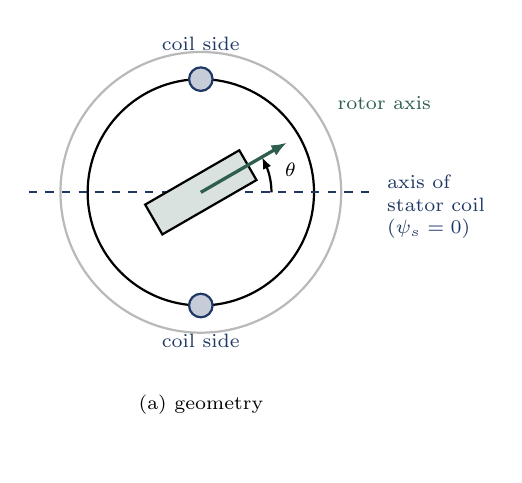
\begin{tikzpicture}[font=\small, x=1.15cm, y=1.15cm, baseline=(cc.base)]
\coordinate (cc) at (0,-2.9);
\draw[thick] (0,0) circle (1.25);
\draw[thick, gray!55] (0,0) circle (1.55);
% stator coil axis (psi_s = 0)
\draw[dashed, thick, fnavy] (-1.9,0) -- (1.9,0);
\node[fnavy, font=\scriptsize, anchor=west, align=left] at (1.95,-0.16)
   {axis of\\stator coil\\($\psi_{s}=0$)};
% coil sides at +-90
\draw[fnavy, fill=fnavy!25, thick] (0,1.25) circle (0.13);
\draw[fnavy, fill=fnavy!25, thick] (0,-1.25) circle (0.13);
\node[fnavy, font=\scriptsize, anchor=south] at (0,1.46) {coil side};
\node[fnavy, font=\scriptsize, anchor=north] at (0,-1.46) {coil side};
% rotor at theta = 30
\begin{scope}[rotate=30]
  \draw[thick, fill=faccent!18] (-0.60,-0.19) rectangle (0.60,0.19);
  \draw[very thick, faccent, -{Latex[length=2mm]}] (0,0) -- (1.10,0);
\end{scope}
\node[faccent, font=\scriptsize, anchor=south west] at (30:1.62) {rotor axis};
% angle arc
\draw[thick,-{Latex[length=1.5mm]}] (0.78,0) arc (0:30:0.78);
\node[font=\scriptsize] at (14:1.02) {$\theta$};
\node[font=\scriptsize] at (0,-2.35) {(a) geometry};
\end{tikzpicture}%
\hspace{0.2cm}%
% ---------- panel (b): developed flux ----------
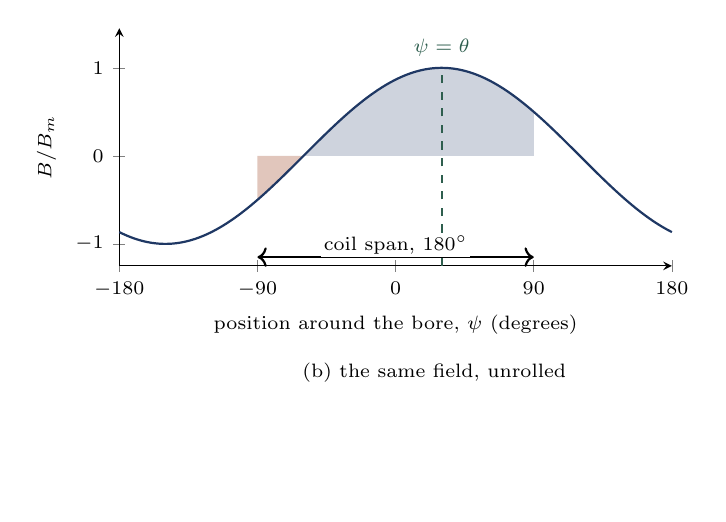
\begin{tikzpicture}[baseline=(bb.base)]
\coordinate (bb) at (0,-2.9);
\begin{axis}[
  width=8.6cm, height=4.6cm,
  xlabel={position around the bore, $\psi$ (degrees)},
  ylabel={$B/B_{m}$},
  xlabel style={font=\scriptsize}, ylabel style={font=\scriptsize},
  domain=-180:180, samples=200,
  xmin=-180, xmax=180, ymin=-1.25, ymax=1.45,
  xtick={-180,-90,0,90,180}, ytick={-1,0,1},
  tick label style={font=\scriptsize},
  axis lines=left, clip=false,
]
% negative part of the window
\addplot[draw=none, fill=fflag!30, domain=-90:-60] {cos(x-30)} \closedcycle;
% positive part of the window
\addplot[draw=none, fill=fnavy!22, domain=-60:90] {cos(x-30)} \closedcycle;
\addplot[thick, fnavy] {cos(x-30)};
\draw[faccent, thick, dashed] (axis cs:30,-1.25) -- (axis cs:30,1.0);
\node[faccent, font=\scriptsize, anchor=south] at (axis cs:30,1.02) {$\psi=\theta$};
\draw[<->, thick] (axis cs:-90,-1.15) -- (axis cs:90,-1.15);
\node[font=\scriptsize, anchor=south, fill=white, inner sep=1pt]
   at (axis cs:0,-1.16) {coil span, $180^\circ$};
\end{axis}
\node[font=\scriptsize] at (4.0,-1.35) {(b) the same field, unrolled};
\end{tikzpicture}
\caption{Where the cosine in \eqref{eq:fluxlink} comes from. The rotor drives
a flux density that varies sinusoidally around the bore, \eqref{eq:airgap}.
The stator coil links whatever lies between its two sides --- the shaded
window in (b). Flux entering the coil (blue) counts positively and flux
leaving it (orange) counts negatively, so the net linkage is the
\emph{signed} area, $2B_{m}\cos(\psi_{s}-\theta)$. Slide the window around
the bore and that signed area traces out a cosine.}
\label{fig:cosine}
\end{figure}

To turn flux linkage into a voltage, use the transformer relation rather than
differentiating \eqref{eq:fluxlink} directly --- it is shorter and it gets the
phase right. Neglecting the resistance and leakage of the rotor winding, the
applied rotor voltage is absorbed entirely by the rate of change of its own
flux linkage:
\[
  v(t)\;\approx\;N_{r}\frac{\mathrm{d}\Phi}{\mathrm{d}t},
  \qquad\text{while}\qquad
  e_{s}(t)=N_{s}\frac{\mathrm{d}\Phi_{s}}{\mathrm{d}t}
          =N_{s}\cos(\psi_{s}-\theta)\frac{\mathrm{d}\Phi}{\mathrm{d}t}.
\]
Dividing one by the other kills the derivative and leaves an algebraic
relation between the two voltages:

\begin{equation}
  \boxed{\;e_{s}(t)=\frac{N_{s}}{N_{r}}\cos(\psi_{s}-\theta)\;v(t)
        =K V_{r}\cos(\psi_{s}-\theta)\sin\omega_{c}t\;}
  \label{eq:onecoil}
\end{equation}

for a rotor excitation $v(t)=V_{r}\sin\omega_{c}t$, with $K=N_{s}/N_{r}$ the
effective turns ratio. Two things are worth noticing before moving on:

\begin{itemize}[leftmargin=1.5em,itemsep=1pt]
\item The \emph{time} behaviour, $\sin\omega_{c}t$, is fixed by the supply and
      is the same in every coil. The coils are in time phase with one another.
\item The \emph{amplitude}, $KV_{r}\cos(\psi_{s}-\theta)$, is the only place
      the shaft angle appears. All the information is in the amplitudes.
\end{itemize}

\begin{keyidea}
A synchro is a \textbf{transformer whose coupling depends on shaft angle}. The
rotor coil is the primary, each stator coil a secondary, and the turns ratio
of each secondary is modulated by $\cos(\psi_{s}-\theta)$. Nothing rotates
electrically and nothing slides in the signal path --- only the coupling
changes.
\end{keyidea}

% ....................................................................
\subsubsection{Step 2 --- three coils, and what appears on the wires}
\label{sss:three}

The stator carries three identical Y-connected coils with their axes
$120^\circ$ apart. Take the axis of $S_{2}$ as the reference, $\psi_{2}=0$,
and place $S_{1}$ at $\psi_{1}=-120^\circ$ and $S_{3}$ at
$\psi_{3}=+120^\circ$. Substituting each $\psi_{k}$ into \eqref{eq:onecoil},
and using $\cos(-x)=\cos x$ throughout, gives the three coil-to-neutral
voltages:

\begin{align}
  v_{s_{1}n}&=KV_{r}\sin\omega_{c}t\,\cos(\theta+120^\circ), \label{eq:v1}\\
  v_{s_{2}n}&=KV_{r}\sin\omega_{c}t\,\cos\theta,             \label{eq:v2}\\
  v_{s_{3}n}&=KV_{r}\sin\omega_{c}t\,\cos(\theta+240^\circ). \label{eq:v3}
\end{align}

(The last one may look odd: $\psi_{3}=+120^\circ$ gives
$\cos(\theta-120^\circ)$, and $\cos(\theta-120^\circ)=\cos(\theta+240^\circ)$
because cosine repeats every $360^\circ$. Nagrath writes it the second way; it
is the same voltage.)

\begin{figure}[H]
\centering
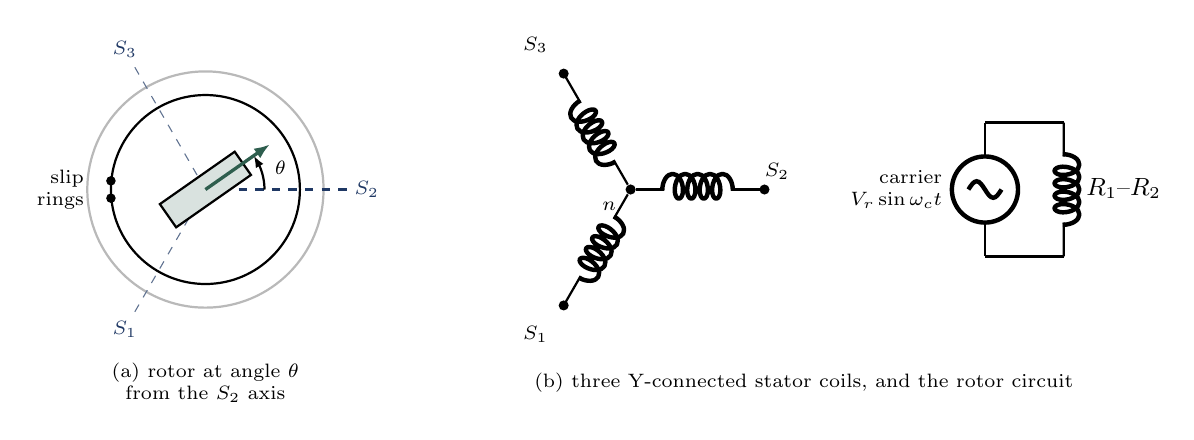
\begin{tikzpicture}[font=\small, x=1cm, y=1cm]
% =================== panel (a): cross-section ===================
\begin{scope}
\draw[thick] (0,0) circle (1.2);
\draw[thick,gray!55] (0,0) circle (1.5);
% three coil axes
\foreach \a/\lb in {0/{$S_{2}$}, 120/{$S_{3}$}, 240/{$S_{1}$}}{
  \draw[dashed, fnavy!70] (0,0) -- (\a:1.80);
  \node[fnavy, font=\scriptsize] at (\a:2.05) {\lb};
}
\draw[dashed, very thick, fnavy] (0,0) -- (0:1.80);
% rotor at 35
\begin{scope}[rotate=35]
  \draw[thick, fill=faccent!18] (-0.58,-0.18) rectangle (0.58,0.18);
  \draw[very thick, faccent, -{Latex[length=2mm]}] (0,0) -- (1.0,0);
\end{scope}
\draw[thick,-{Latex[length=1.5mm]}] (0.75,0) arc (0:35:0.75);
\node[font=\scriptsize] at (16:0.99) {$\theta$};
% slip rings
\draw[fill] (-1.20,0.11) circle (1.5pt);
\draw[fill] (-1.20,-0.11) circle (1.5pt);
\node[font=\scriptsize, anchor=east, align=right] at (-1.42,0) {slip\\rings};
\node[font=\scriptsize, align=center] at (0,-2.45)
   {(a) rotor at angle $\theta$\\from the $S_{2}$ axis};
\end{scope}
% =================== panel (b): Y-connection ===================
\begin{scope}[shift={(5.4,0)}]
\node[circle,fill,inner sep=1.3pt] (N) at (0,0) {};
\node[font=\scriptsize, anchor=north east] at (-0.06,-0.04) {$n$};
\foreach \a/\lb/\pos in {0/{$S_{2}$}/{above}, 120/{$S_{3}$}/{above left},
                         240/{$S_{1}$}/{below left}}{
  \coordinate (T\a) at (\a:1.7);
  \draw[thick] (N) to[L] (T\a);
  \draw[fill] (T\a) circle (1.6pt);
  \node[font=\scriptsize, \pos] at (\a:1.86) {\lb};
}
\end{scope}
% =================== panel (b): rotor circuit ===================
\begin{scope}[shift={(9.9,0)}]
  \draw[thick] (1.0,0.85) to[L={$R_{1}$--$R_{2}$}] (1.0,-0.85);
  \draw[thick] (1.0,0.85) -- (0,0.85);
  \draw[thick] (1.0,-0.85) -- (0,-0.85);
  \draw[thick] (0,0.85) to[sV] (0,-0.85);
  \node[font=\scriptsize, anchor=east, align=right] at (-0.42,0)
     {carrier\\$V_{r}\sin\omega_{c}t$};
\end{scope}
% caption for the right-hand pair, centred over its span
\node[font=\scriptsize, align=center] at (7.6,-2.45)
   {(b) three Y-connected stator coils, and the rotor circuit};
\end{tikzpicture}
\caption{The synchro transmitter. (a) Mechanically, three coil axes
$120^\circ$ apart and a rotor at angle $\theta$, measured from the $S_{2}$
axis. (b) Electrically, three Y-connected secondaries and one rotating
primary $R_{1}$--$R_{2}$ fed through slip rings. Cf.\ Nagrath \& Gopal
Figs.~4.10--4.11, pp.~92--93. Note that only three wires leave the stator:
the neutral $n$ is internal and is not brought out.}
\label{fig:transmitter}
\end{figure}

\paragraph{What is actually measurable.} The neutral $n$ is buried inside the
machine. Only three wires leave it, so the voltages you can measure are the
three \emph{line-to-line} voltages, and these are differences of
\eqref{eq:v1}--\eqref{eq:v3}. Take the first, and use the identity
$\cos A-\cos B=-2\sin\frac{A+B}{2}\sin\frac{A-B}{2}$:
\begin{align*}
  v_{s_{1}s_{2}}&=v_{s_{1}n}-v_{s_{2}n}
   =KV_{r}\sin\omega_{c}t\big[\cos(\theta+120^\circ)-\cos\theta\big]\\
  &=KV_{r}\sin\omega_{c}t\big[-2\sin(\theta+60^\circ)\sin 60^\circ\big]
   =-\sqrt{3}\,KV_{r}\sin(\theta+60^\circ)\sin\omega_{c}t,
\end{align*}
and since $-\sin x=\sin(x+180^\circ)$, this is the form Nagrath quotes. Doing
the same for the other two pairs:

\begin{align}
  v_{s_{1}s_{2}}&=\sqrt{3}\,KV_{r}\sin(\theta+240^\circ)\sin\omega_{c}t, \label{eq:l1}\\
  v_{s_{2}s_{3}}&=\sqrt{3}\,KV_{r}\sin(\theta+120^\circ)\sin\omega_{c}t, \label{eq:l2}\\
  v_{s_{3}s_{1}}&=\sqrt{3}\,KV_{r}\sin\theta\,\sin\omega_{c}t.           \label{eq:l3}
\end{align}

Two checks are worth making on \eqref{eq:v1}--\eqref{eq:v3} before going on.

\smallskip
\textbf{Check 1: the three coil voltages sum to zero.} Adding
\eqref{eq:v1}--\eqref{eq:v3},
\[
  \cos(\theta+120^\circ)+\cos\theta+\cos(\theta+240^\circ)=0
  \qquad\text{for every }\theta,
\]
which is the standard result that three equal phasors $120^\circ$ apart
cancel. That is why the Y point needs no return wire: whatever currents these
voltages drive, Kirchhoff's current law at $n$ is satisfied without one.

\smallskip
\textbf{Check 2: the electrical zero.} Put $\theta=0$. Then $S_{2}$ carries
its maximum voltage (its axis faces the rotor squarely) and, from
\eqref{eq:l3}, the line voltage $v_{s_{3}s_{1}}$ is exactly zero. This
position is the \textbf{electrical zero} of the transmitter, and it is the
reference against which shaft angle is quoted. It is easy to find in practice:
turn the shaft until $v_{s_{3}s_{1}}$ nulls.

\begin{figure}[H]
\centering
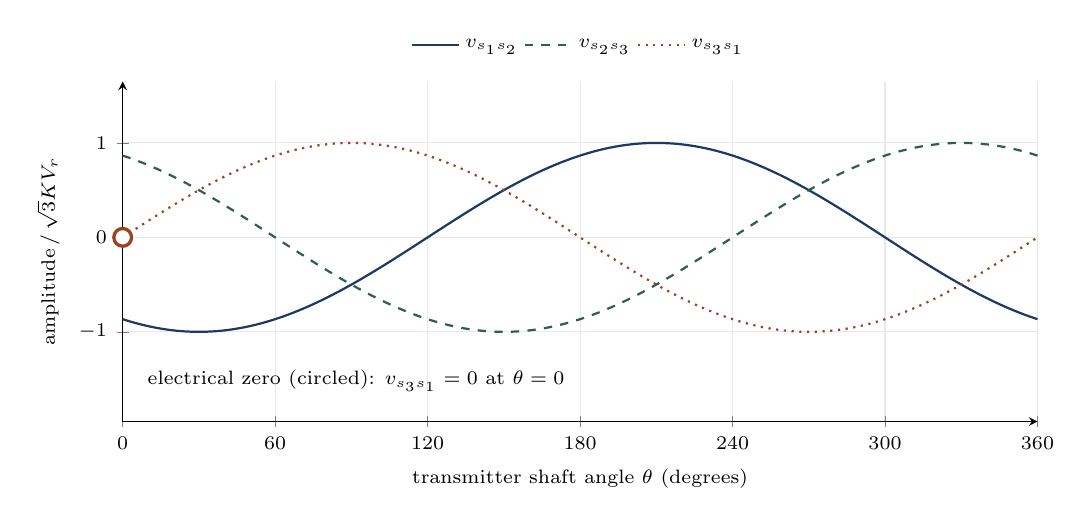
\begin{tikzpicture}
\begin{axis}[
  width=13.2cm, height=5.9cm,
  xlabel={transmitter shaft angle $\theta$ (degrees)},
  ylabel={amplitude\,/\,$\sqrt{3}KV_{r}$},
  xlabel style={font=\scriptsize}, ylabel style={font=\scriptsize},
  domain=0:360, samples=241,
  xmin=0, xmax=360, ymin=-1.95, ymax=1.65,
  xtick={0,60,...,360}, ytick={-1,0,1},
  tick label style={font=\scriptsize},
  grid=both, grid style={gray!18},
  legend style={font=\scriptsize, at={(0.5,1.16)}, anchor=north, legend columns=3, draw=none},
  axis lines=left, clip=false,
]
\addplot[thick, fnavy]           {sin(x+240)}; \addlegendentry{$v_{s_{1}s_{2}}$}
\addplot[thick, faccent, dashed] {sin(x+120)}; \addlegendentry{$v_{s_{2}s_{3}}$}
\addplot[thick, fflag, dotted]   {sin(x)};     \addlegendentry{$v_{s_{3}s_{1}}$}
\draw[fflag, very thick, fill=white] (axis cs:0,0) circle (3.2pt);
\node[font=\scriptsize, anchor=west] at (axis cs:6,-1.52)
   {electrical zero (circled): $v_{s_{3}s_{1}}=0$ at $\theta=0$};
\end{axis}
\end{tikzpicture}
\caption{The three line voltages of \eqref{eq:l1}--\eqref{eq:l3} as the
transmitter shaft turns. No two shaft angles in a full revolution give the
same set of three amplitudes-with-signs, so the three wires carry an
unambiguous code for $\theta$. This is why a synchro can also be used on its
own as a position \emph{transmitter}, not only inside an error detector.}
\label{fig:linev}
\end{figure}

% ....................................................................
\subsubsection{Step 3 --- rebuilding the flux in the second machine}
\label{sss:rebuild}

Now wire those three stator terminals to the three stator terminals of a
second machine, the \textbf{synchro control transformer}. It is built like the
transmitter except for its rotor, which is cylindrical --- more on that below.

Currents circulate in the two sets of stator windings. If the resistances and
leakage reactances are small, the current in each phase of the control
transformer is very nearly proportional to the voltage impressed on it, so
phase $k$ of the control transformer carries a current
$i_{k}\propto\cos(\theta-\psi_{k})$ --- the same pattern of amplitudes the
transmitter had. Each of those currents drives a magnetomotive force
\emph{along its own coil axis}, and the three add.

This is where the machine actually works, so it is worth doing properly rather
than asserting. Write the m.m.f.\ of phase $k$ as a vector of length
$\cos(\theta-\psi_{k})$ pointing along $\hat{u}(\psi_{k})
=(\cos\psi_{k},\,\sin\psi_{k})$, and sum over the three phases
$\psi_{k}\in\{-120^\circ,\,0,\,+120^\circ\}$. Take the horizontal component
first, using $\cos A\cos B=\tfrac{1}{2}[\cos(A-B)+\cos(A+B)]$:
\[
  \sum_{k}\cos(\theta-\psi_{k})\cos\psi_{k}
  =\frac{1}{2}\sum_{k}\cos\theta+\frac{1}{2}\sum_{k}\cos(\theta-2\psi_{k})
  =\frac{3}{2}\cos\theta+0 .
\]
The second sum vanishes because doubling three angles $120^\circ$ apart gives
three angles that are again $120^\circ$ apart, and those cancel as in Check~1.
The vertical component goes the same way and yields $\tfrac{3}{2}\sin\theta$.
So

\begin{equation}
  \mathbf{F}_{\text{total}}
  =\sum_{k}\cos(\theta-\psi_{k})\,\hat{u}(\psi_{k})
  =\frac{3}{2}\,\hat{u}(\theta).
  \label{eq:mmf}
\end{equation}

\begin{keyidea}
Equation~\eqref{eq:mmf} is the synchro. Three stationary coils, carrying
currents in the ratio $\cos(\theta-\psi_{k})$, produce between them a single
resultant field pointing along the direction $\theta$ --- \emph{whatever}
$\theta$ is, and with a magnitude $\tfrac{3}{2}$ that does not depend on
$\theta$ either. The control transformer therefore contains a copy of the
transmitter's flux, pointing the same way, with no moving part having carried
it there.
\end{keyidea}

\begin{figure}[H]
\centering
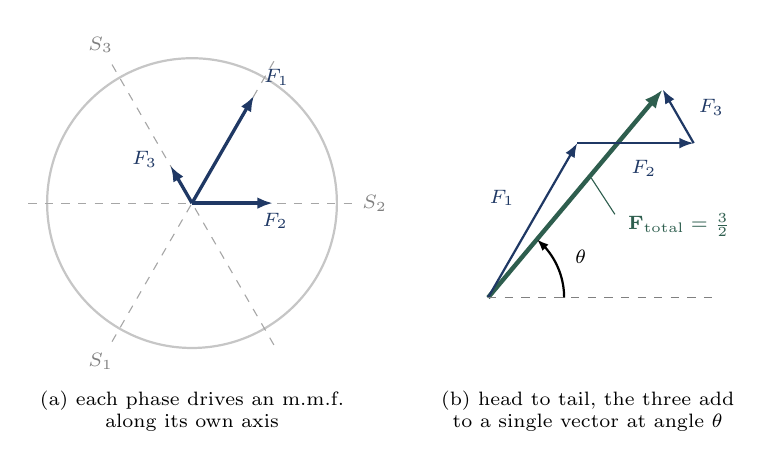
\begin{tikzpicture}[font=\small, x=1.6cm, y=1.6cm]
% ---------- left: the three components ----------
\begin{scope}
\draw[thick, gray!45] (0,0) circle (1.15);
\foreach \a/\lb in {0/{$S_{2}$}, 120/{$S_{3}$}, 240/{$S_{1}$}}{
  \draw[dashed, gray!70] (\a-180:1.3) -- (\a:1.3);
  \node[gray, font=\scriptsize] at (\a:1.45) {\lb};
}
% components for theta = 50 deg: F1=-0.9848 along 240 -> points at 60
\draw[fnavy, very thick, -{Latex[length=2mm]}] (0,0) -- (60:0.985);
\node[fnavy, font=\scriptsize, anchor=south west] at (60:0.99) {$F_{1}$};
\draw[fnavy, very thick, -{Latex[length=2mm]}] (0,0) -- (0:0.643);
\node[fnavy, font=\scriptsize, anchor=north] at (0:0.66) {$F_{2}$};
\draw[fnavy, very thick, -{Latex[length=2mm]}] (0,0) -- (120:0.342);
\node[fnavy, font=\scriptsize, anchor=east] at (120:0.40) {$F_{3}$};
\node[font=\scriptsize, align=center] at (0,-1.65)
   {(a) each phase drives an m.m.f.\\along its own axis};
\end{scope}
% ---------- right: head to tail ----------
\begin{scope}[shift={(2.35,-0.75)}, x=2.3cm, y=2.3cm]
\coordinate (O)  at (0,0);
\coordinate (P1) at (0.4924,0.8529);
\coordinate (P2) at (1.1352,0.8529);
\coordinate (P3) at (0.9642,1.1491);
\draw[faccent, ultra thick, -{Latex[length=2.4mm]}] (O) -- (P3);
\draw[fnavy, thick, -{Latex[length=1.8mm]}] (O)  -- (P1);
\draw[fnavy, thick, -{Latex[length=1.8mm]}] (P1) -- (P2);
\draw[fnavy, thick, -{Latex[length=1.8mm]}] (P2) -- (P3);
\node[fnavy, font=\scriptsize, anchor=east]  at (0.20,0.55) {$F_{1}$};
\node[fnavy, font=\scriptsize, anchor=north] at (0.86,0.81) {$F_{2}$};
\node[fnavy, font=\scriptsize, anchor=west]  at (1.11,1.05) {$F_{3}$};
\node[faccent, font=\scriptsize, anchor=west, align=left]
   at (0.72,0.40) {$\mathbf{F}_{\text{total}}=\tfrac{3}{2}$};
\draw[faccent, thin] (0.70,0.46) -- (0.57,0.66);
\draw[dashed, gray] (O) -- (1.25,0);
\draw[thick,-{Latex[length=1.5mm]}] (0.42,0) arc (0:50:0.42);
\node[font=\scriptsize] at (24:0.56) {$\theta$};
\node[font=\scriptsize, align=center] at (0.55,-0.626)
   {(b) head to tail, the three add\\to a single vector at angle $\theta$};
\end{scope}
\end{tikzpicture}
\caption{Equation~\eqref{eq:mmf} drawn, for $\theta=50^\circ$. In (a),
$F_{1}=\cos170^\circ$ is negative, so it points \emph{opposite} to the
$S_{1}$ axis. Adding the three head to tail in (b) gives a resultant of length
$\tfrac{3}{2}$ lying exactly along $\theta$. Repeat the construction for any
other $\theta$ and the same two facts hold --- that constancy of length and
fidelity of direction is what makes the device useful.}
\label{fig:mmf}
\end{figure}

\begin{pitfall}
The resultant in \eqref{eq:mmf} is a \emph{stationary} field whose magnitude
pulsates at the carrier frequency; it is not a rotating field. Do not carry
over the rotating-field picture from three-phase induction machines. There,
the three currents are $120^\circ$ apart \emph{in time} and the resultant
sweeps round the bore. Here the three currents are in time phase with one
another --- all of them follow the same $\sin\omega_{c}t$ --- and only their
\emph{amplitudes} differ, so the resultant stands still and pulsates. The
direction it stands in is set by the shaft, not by time.
\end{pitfall}

\paragraph{Two construction details, and why they are there.} The control
transformer differs from the transmitter in two respects, both deliberate.

\begin{itemize}[leftmargin=1.5em,itemsep=2pt]
\item \textbf{Its rotor is cylindrical}, giving a uniform air gap. The rotor
      of the transmitter is dumb-bell shaped, which is fine because nothing is
      connected to it but the supply. The control transformer rotor, however,
      feeds an amplifier, and if the air gap changed as the shaft turned then
      so would the rotor's output impedance --- and with it the gain of the
      amplifier stage. A uniform gap keeps the source impedance seen by the
      amplifier constant at every shaft angle.
\item \textbf{Its stator has a higher impedance per phase}, so it draws less
      current from the transmitter. That allows several control transformers
      to be driven from one transmitter --- one shaft angle distributed to
      several loops.
\end{itemize}

% ....................................................................
\subsubsection{Step 4 --- the output voltage, and the $90^\circ$ offset}
\label{sss:output}

Inside the control transformer there is now a pulsating flux lying along the
direction $\theta$. Its rotor is a coil sitting in that flux, so step~1
applies again, unchanged. If $\phi$ is the angle between the control
transformer's rotor axis and the flux axis, then by \eqref{eq:onecoil}

\begin{equation}
  e(t)=K'V_{r}\cos\phi\,\sin\omega_{c}t.
  \label{eq:ct}
\end{equation}

All that remains is to express $\phi$ in terms of the two shaft angles we
care about. Let $\theta$ be the transmitter shaft angle from \emph{its}
electrical zero, and $\alpha$ the control transformer shaft angle from
\emph{its} zero, both measured in the same sense. The flux inside the control
transformer lies at $\theta$ from its $S_{2}$ axis. The control transformer's
rotor is mounted so that at $\alpha=0$ it sits at $90^\circ$ to that axis, and
turning its shaft by $\alpha$ carries it to $90^\circ+\alpha$. The angle
between rotor and flux is therefore

\begin{equation}
  \phi=(90^\circ+\alpha)-\theta=90^\circ-(\theta-\alpha),
  \label{eq:phi}
\end{equation}

and substituting \eqref{eq:phi} into \eqref{eq:ct}, with
$\cos(90^\circ-x)=\sin x$:

\begin{equation}
  \boxed{\;e(t)=K'V_{r}\,\sin(\theta-\alpha)\,\sin\omega_{c}t\;}
  \label{eq:synchro}
\end{equation}

\begin{figure}[H]
\centering
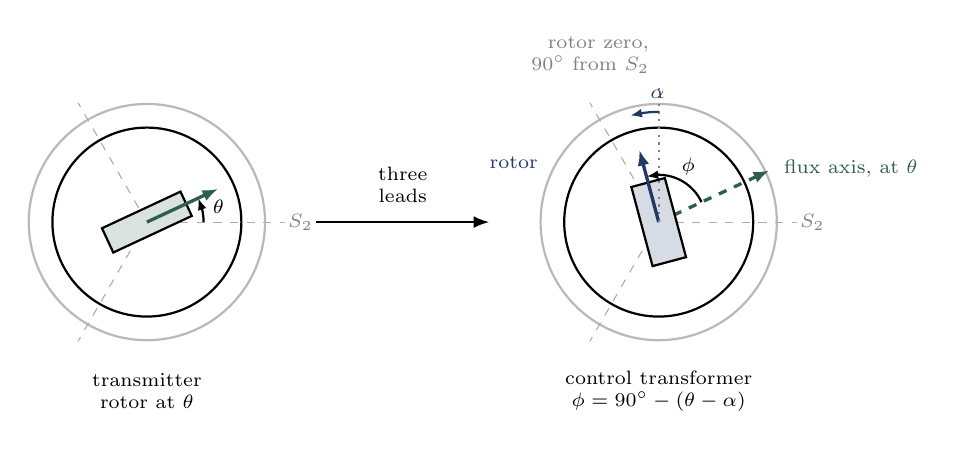
\begin{tikzpicture}[font=\small, x=1cm, y=1cm]
% ---------- transmitter ----------
\begin{scope}
\draw[thick] (0,0) circle (1.2);
\draw[thick,gray!55] (0,0) circle (1.5);
\foreach \a in {0,120,240}{\draw[dashed, gray!65] (0,0) -- (\a:1.75);}
\node[gray, font=\scriptsize] at (0:1.95) {$S_{2}$};
\begin{scope}[rotate=25]
  \draw[thick, fill=faccent!18] (-0.55,-0.17) rectangle (0.55,0.17);
  \draw[very thick, faccent, -{Latex[length=2mm]}] (0,0) -- (1.0,0);
\end{scope}
\draw[thick,-{Latex[length=1.5mm]}] (0.72,0) arc (0:25:0.72);
\node[font=\scriptsize] at (12:0.93) {$\theta$};
\node[font=\scriptsize, align=center] at (0,-2.15) {transmitter\\rotor at $\theta$};
\end{scope}
% ---------- link ----------
\draw[thick, -{Latex[length=2mm]}] (2.15,0) -- (4.35,0);
\node[font=\scriptsize, align=center, anchor=south] at (3.25,0.12)
   {three\\leads};
% ---------- control transformer ----------
\begin{scope}[shift={(6.5,0)}]
\draw[thick] (0,0) circle (1.2);
\draw[thick,gray!55] (0,0) circle (1.5);
\foreach \a in {0,120,240}{\draw[dashed, gray!65] (0,0) -- (\a:1.75);}
\node[gray, font=\scriptsize] at (0:1.95) {$S_{2}$};
% flux axis at theta = 25
\draw[very thick, faccent, dashed, -{Latex[length=2mm]}] (0,0) -- (25:1.55);
\node[faccent, font=\scriptsize, anchor=west] at (25:1.62) {flux axis, at $\theta$};
% rotor at 90 + alpha, alpha = 15  -> 105
\begin{scope}[rotate=105]
  \draw[thick, fill=fnavy!18] (-0.52,-0.22) rectangle (0.52,0.22);
  \draw[very thick, fnavy, -{Latex[length=2mm]}] (0,0) -- (0.95,0);
\end{scope}
\node[fnavy, font=\scriptsize, anchor=east] at (152:1.60) {rotor};
% the CT rotor's own electrical zero, 90 deg from S2
\draw[dotted, thick, gray] (0,0) -- (90:1.72);
\node[gray, font=\scriptsize, anchor=south east, align=right] at (90:1.76)
   {rotor zero,\\$90^\circ$ from $S_{2}$};
% alpha arc from 90 to 105
\draw[fnavy, thick,-{Latex[length=1.5mm]}] (90:1.40) arc (90:105:1.40);
\node[fnavy, font=\scriptsize, anchor=south west] at (99:1.46) {$\alpha$};
% phi arc from 25 to 105
\draw[thick,-{Latex[length=1.5mm]}] (25:0.60) arc (25:105:0.60);
\node[font=\scriptsize] at (62:0.80) {$\phi$};
\node[font=\scriptsize, align=center] at (0,-2.15)
   {control transformer\\$\phi=90^\circ-(\theta-\alpha)$};
\end{scope}
\end{tikzpicture}
\caption{The geometry behind \eqref{eq:phi}, drawn for $\theta=25^\circ$ and
$\alpha=15^\circ$, so $\phi=80^\circ$. The transmitter's rotor angle is
reproduced as the direction of the flux inside the control transformer; the
control transformer's own rotor is mounted a further $90^\circ$ round.
Cf.\ Nagrath \& Gopal Fig.~4.12, p.~94.}
\label{fig:pair}
\end{figure}

\paragraph{Why mount the rotor at $90^\circ$?} It looks like an odd choice
until you ask what an error detector must do. Two properties are wanted, and
$\phi=90^\circ$ delivers both at once.

\begin{itemize}[leftmargin=1.5em,itemsep=2pt]
\item \textbf{It must read zero when the error is zero.} A summing junction
      that outputs something when $r=c$ is not a summing junction. From
      \eqref{eq:ct}, $\cos\phi=0$ exactly at $\phi=90^\circ$, so the offset
      puts the null where the shafts agree.
\item \textbf{It must be most sensitive there.} Differentiating
      \eqref{eq:ct}, the change in output per unit change in angle is
      $|\mathrm{d}e/\mathrm{d}\phi|\propto|\sin\phi|$, which is
      \emph{largest} at $\phi=90^\circ$. The null and the point of maximum
      slope coincide.
\end{itemize}

Had the rotor been aligned with the flux instead, at $\phi=0$, the output
would sit at its maximum, the slope would be zero, and small shaft errors
would produce almost no change in output --- and no sign information at all,
since $\cos$ is even. The device would be useless as an error detector. A
sensor for a feedback loop should always be arranged to work about a null,
and this is a clean example of why.

% ....................................................................
\subsubsection{Step 5 --- linearising, and what it costs}
\label{sss:linear}

Equation~\eqref{eq:synchro} is exact, but $\sin(\theta-\alpha)$ is not a gain.
For small shaft differences, $\sin x\approx x$, and

\begin{equation}
  e(t)\;\approx\;K_{s}\,(\theta-\alpha)\,\sin\omega_{c}t,
  \qquad K_{s}=K'V_{r},\qquad [K_{s}]=\si{\volt\per\radian},
  \label{eq:linear}
\end{equation}

where $K_{s}$ is the \textbf{sensitivity of the error detector}. Now the pair
is a pure gain from shaft-angle difference to signal amplitude --- exactly the
$\otimes$ of the block diagram, followed by a constant.

\begin{figure}[H]
\centering
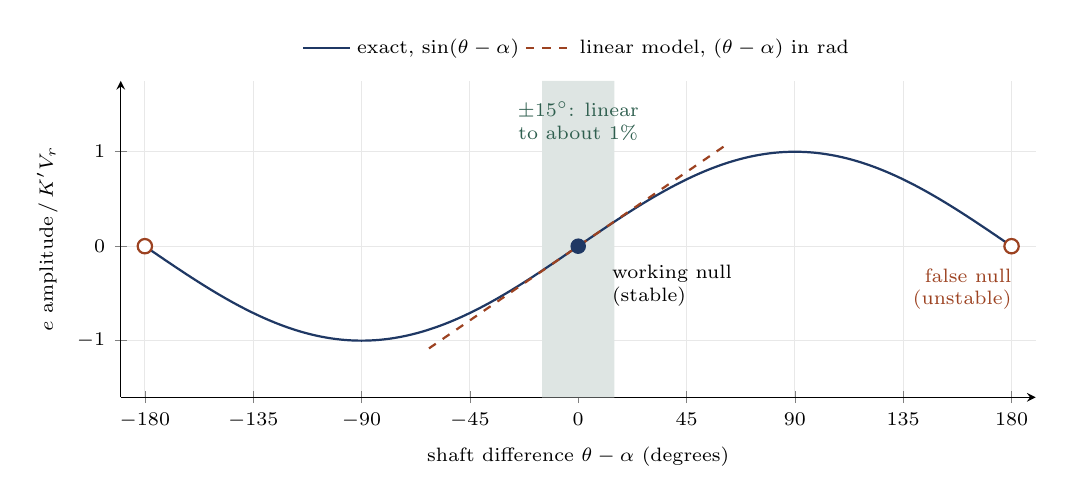
\begin{tikzpicture}
\begin{axis}[
  width=13.2cm, height=5.6cm,
  xlabel={shaft difference $\theta-\alpha$ (degrees)},
  ylabel={$e$ amplitude\,/\,$K'V_{r}$},
  xlabel style={font=\scriptsize}, ylabel style={font=\scriptsize},
  xmin=-190, xmax=190, ymin=-1.6, ymax=1.75,
  xtick={-180,-135,...,180}, ytick={-1,0,1},
  tick label style={font=\scriptsize},
  grid=both, grid style={gray!18},
  axis lines=left, clip=false,
  legend style={font=\scriptsize, at={(0.5,1.17)}, anchor=north,
                legend columns=2, draw=none},
]
\addplot[draw=none, fill=faccent!16, forget plot] coordinates
  {(-15,-1.6) (15,-1.6) (15,1.75) (-15,1.75)} \closedcycle;
\addplot[thick, fnavy, domain=-180:180, samples=241] {sin(x)};
\addlegendentry{exact, $\sin(\theta-\alpha)$}
\addplot[thick, fflag, dashed, domain=-62:62, samples=2] {x*pi/180};
\addlegendentry{linear model, $(\theta-\alpha)$ in rad}
\draw[fnavy, fill=fnavy] (axis cs:0,0) circle (2.6pt);
\draw[fflag, thick, fill=white] (axis cs:180,0) circle (2.6pt);
\draw[fflag, thick, fill=white] (axis cs:-180,0) circle (2.6pt);
\node[font=\scriptsize, anchor=north west, align=left] at (axis cs:10,-0.10)
  {working null\\(stable)};
\node[font=\scriptsize, fflag, anchor=north east, align=right] at (axis cs:184,-0.14)
  {false null\\(unstable)};
\node[font=\scriptsize, faccent, anchor=south, align=center] at (axis cs:0,1.02)
  {$\pm15^\circ$: linear\\to about 1\%};
\end{axis}
\end{tikzpicture}
\caption{The exact characteristic \eqref{eq:synchro} against the linear model
\eqref{eq:linear}. Inside the shaded band the two are indistinguishable at the
accuracy of any real measurement; a servo drives the error into that band and
keeps it there, so the linear model is not a compromise so much as a
description of where the device actually lives.}
\label{fig:sine}
\end{figure}

\paragraph{How small is small?} The relative error of $\sin x\approx x$ is
worth knowing as a number rather than a feeling:

\begin{center}
\begin{tabular}{lcccccc}
\toprule
$\theta-\alpha$        & $5^\circ$ & $10^\circ$ & $14^\circ$ & $15^\circ$ & $20^\circ$ & $30^\circ$ \\
\midrule
error in $e$ & 0.13\% & 0.51\% & 1.0\% & 1.15\% & 2.1\% & 4.7\% \\
\bottomrule
\end{tabular}
\end{center}

So the linear model is good to about 1\% out to $\pm14^\circ$ and to about 5\%
out to $\pm30^\circ$. In a position servo, whose whole purpose is to hold
$\theta-\alpha$ near zero, the steady-state error is a small fraction of a
degree and the approximation is far better than any other in the loop.

\begin{pitfall}
$\sin(\theta-\alpha)$ is also zero at $\theta-\alpha=180^\circ$. That is a
\emph{false null}: the pair produces no output there even though the shafts
are as far apart as they can be. It is not, however, a place the servo can
settle. Just past it, at $\theta-\alpha=180^\circ+\delta$, the exact output is
$\sin(180^\circ+\delta)=-\sin\delta$ --- the \emph{opposite} sign to what the
linear model predicts. The feedback that should pull the shaft back instead
pushes it away, so the $180^\circ$ point is an unstable equilibrium and the
loop runs off it towards the true null. A synchro pair therefore cannot tell
you absolute position over a whole revolution, but as an error detector inside
a loop it does not need to.
\end{pitfall}

\begin{pitfall}
Watch the units in which $K_{s}$ is quoted. Nagrath gives it in
volts~(rms) per radian, so read $V_{r}$ as the \emph{rms} rotor voltage and
treat $\sin\omega_{c}t$ as a marker of the carrier's frequency and phase
rather than as a literal peak-value multiplier. Take $V_{r}$ to be the peak
value instead and $K_{s}$ comes out $\sqrt{2}$ times larger. Both conventions
appear on datasheets; settle which one you are in before putting a number into
a loop gain, because a stray $\sqrt{2}$ in the forward path is a real error in
the damping you predict.
\end{pitfall}

\begin{workedex}[breakable, title={Worked example 1.1 --- sizing a synchro error detector}]
A control transformer is quoted as producing \SI{22.5}{\volt} rms at its rotor
terminals at maximum coupling, from a \SI{26}{\volt}, \SI{400}{\hertz} carrier
supply.

\smallskip
\textbf{(a) What is its sensitivity?} Maximum coupling is $\phi=0$ --- rotor
aligned with the flux --- which by \eqref{eq:phi} means the shafts differ by
$90^\circ$, so $\sin(\theta-\alpha)=1$ and the whole of $K'V_{r}$ appears:
\[
  K_{s}=\SI{22.5}{\volt\per\radian}
       =\frac{22.5\times\pi}{180}=\SI{0.393}{\volt}\ \text{per degree}.
\]

\textbf{(b) What comes out at a \SI{2}{\degree} shaft error?} Exactly, from
\eqref{eq:synchro},
\[
  e_{\text{rms}}=22.5\sin 2^\circ=22.5\times0.034899=\SI{0.785}{\volt}.
\]
From the linear model \eqref{eq:linear}, with
$2^\circ=\SI{0.034907}{\radian}$,
\[
  e_{\text{rms}}\approx22.5\times0.034907=\SI{0.785}{\volt}.
\]
The two agree to four figures; the error of linearisation here is 0.02\%,
which is two orders of magnitude below the tolerance of the components around
it.

\smallskip
\textbf{(c) What does the amplifier have to cope with?} If the loop can be
disturbed by as much as $30^\circ$ before the servo catches it, the detector
will momentarily put out $22.5\sin30^\circ=\SI{11.3}{\volt}$ rms. An amplifier
sized on the linear model alone would have predicted
$22.5\times0.5236=\SI{11.8}{\volt}$ --- close enough for sizing, but note that
the \emph{exact} value is the smaller one. Linearisation always over-estimates
the signal, never under-estimates it, because $\sin x<x$.
\end{workedex}

% ....................................................................
\subsubsection{Reading the output: a modulated carrier}
\label{sss:carrier}

Equation \eqref{eq:linear} has an unfamiliar shape. It is not a voltage
proportional to the error; it is a \emph{carrier} $\sin\omega_{c}t$ whose
amplitude is proportional to the error. Let the shafts move, so that
$\theta-\alpha$ becomes a slowly varying function of time. Then
\[
  e(t)=\underbrace{K_{s}\big[\theta(t)-\alpha(t)\big]}_{\text{modulating signal, slow}}
       \times\underbrace{\sin\omega_{c}t}_{\text{carrier, fast}} .
\]
This is \textbf{suppressed-carrier modulation}, and it has two properties that
matter for reading an oscilloscope and for designing the rest of the loop.

\begin{itemize}[leftmargin=1.5em,itemsep=2pt]
\item \textbf{No error, no signal.} When $\theta=\alpha$ the output is
      identically zero --- the carrier itself is absent. Compare ordinary
      amplitude modulation, in which the carrier is still there at full
      strength when the modulating signal is zero. Here the carrier is
      \emph{suppressed}, hence the name.
\item \textbf{The sign lives in the phase.} When $\theta-\alpha$ changes sign,
      the amplitude factor changes sign, and multiplying $\sin\omega_{c}t$ by
      a negative number is the same as shifting it by $180^\circ$. The
      envelope of $e(t)$ is $|\,K_{s}(\theta-\alpha)|$ and carries no sign; the
      sign is carried entirely by whether $e(t)$ is in phase or antiphase with
      the supply.
\end{itemize}

\begin{figure}[H]
\centering
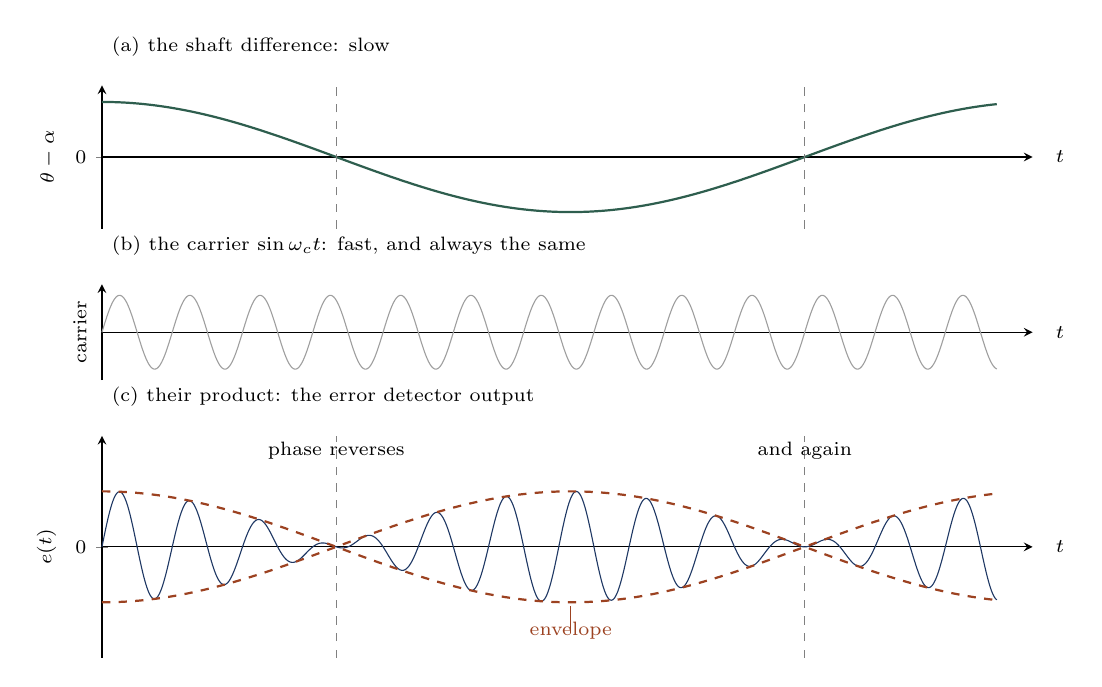
\begin{tikzpicture}
% ---- (a) the modulating signal ----
\begin{axis}[name=ax1,
  width=13.4cm, height=3.4cm,
  ylabel={$\theta-\alpha$}, ylabel style={font=\scriptsize},
  title={(a) the shaft difference: slow},
  title style={font=\scriptsize, at={(0,1)}, anchor=south west, yshift=1pt},
  domain=0:10, samples=300,
  xmin=0, xmax=10.4, ymin=-1.3, ymax=1.3,
  xtick=\empty, ytick={0},
  tick label style={font=\scriptsize},
  axis x line=middle, axis y line=left, clip=false,
]
\addplot[thick, faccent] {cos(deg(0.6*x))};
\node[font=\scriptsize, anchor=west] at (axis cs:10.55,0) {$t$};
\draw[gray, dashed] (axis cs:2.618,-1.3) -- (axis cs:2.618,1.3);
\draw[gray, dashed] (axis cs:7.854,-1.3) -- (axis cs:7.854,1.3);
\end{axis}
% ---- (b) the carrier ----
\begin{axis}[name=ax2, at={(ax1.below south west)}, anchor=north west, yshift=-7mm,
  width=13.4cm, height=2.8cm,
  ylabel={carrier}, ylabel style={font=\scriptsize},
  title={(b) the carrier $\sin\omega_{c}t$: fast, and always the same},
  title style={font=\scriptsize, at={(0,1)}, anchor=south west, yshift=1pt},
  domain=0:10, samples=900,
  xmin=0, xmax=10.4, ymin=-1.3, ymax=1.3,
  xtick=\empty, ytick=\empty,
  axis x line=middle, axis y line=left, clip=false,
]
\addplot[thin, gray!75] {sin(deg(8*x))};
\node[font=\scriptsize, anchor=west] at (axis cs:10.55,0) {$t$};
\end{axis}
% ---- (c) the product ----
\begin{axis}[name=ax3, at={(ax2.below south west)}, anchor=north west, yshift=-7mm,
  width=13.4cm, height=4.4cm,
  ylabel={$e(t)$}, ylabel style={font=\scriptsize},
  title={(c) their product: the error detector output},
  title style={font=\scriptsize, at={(0,1)}, anchor=south west, yshift=1pt},
  domain=0:10, samples=900,
  xmin=0, xmax=10.4, ymin=-2.0, ymax=2.0,
  xtick=\empty, ytick={0},
  tick label style={font=\scriptsize},
  axis x line=middle, axis y line=left, clip=false,
]
\addplot[thin, fnavy] {cos(deg(0.6*x))*sin(deg(8*x))};
\addplot[thick, fflag, dashed, samples=300] {abs(cos(deg(0.6*x)))};
\addplot[thick, fflag, dashed, samples=300] {-abs(cos(deg(0.6*x)))};
\draw[gray, dashed] (axis cs:2.618,-2.0) -- (axis cs:2.618,2.0);
\draw[gray, dashed] (axis cs:7.854,-2.0) -- (axis cs:7.854,2.0);
\node[font=\scriptsize, fflag, anchor=south] at (axis cs:5.24,-1.85) {envelope};
\draw[fflag, thin] (axis cs:5.24,-1.55) -- (axis cs:5.24,-1.06);
\node[font=\scriptsize, anchor=south, align=center] at (axis cs:2.618,1.40)
   {phase reverses};
\node[font=\scriptsize, anchor=south, align=center] at (axis cs:7.854,1.40)
   {and again};
\node[font=\scriptsize, anchor=west] at (axis cs:10.55,0) {$t$};
\end{axis}
\end{tikzpicture}
\caption{Suppressed-carrier modulation at the output of the synchro pair.
Cf.\ Nagrath \& Gopal Fig.~4.13, p.~95. Where the shaft difference passes
through zero (dashed lines) the output vanishes and then comes back
\emph{inverted} relative to the carrier. The envelope alone (orange) is the
same on both sides of that crossing: it gives the size of the error but not
its direction.}
\label{fig:carrier}
\end{figure}

\begin{pitfall}
In a carrier system the information is in the \textbf{envelope and its
phase}, never in the instantaneous value. A student who reads the error
straight off an oscilloscope trace of $e(t)$ will conclude that the error is
swinging violently at \SI{400}{\hertz} while the shaft stands perfectly still.
Trigger the scope on the carrier supply and look at the envelope instead ---
and note which way up the trace is, because that is the sign of the error.
\end{pitfall}

\paragraph{Two consequences for the rest of the loop.} First, since the sign
lives in the phase, whatever comes next must be \emph{phase-sensitive} --- a
simple rectifier would deliver $|\theta-\alpha|$ and the loop would drive the
shaft the wrong way half the time. In the a.c.\ position control systems of
\S\ref{sec:synchro} this is arranged elegantly: the a.c.\ servomotor's
reference phase is fed from the same carrier supply as the synchro rotor, so
the motor itself compares the two phases and turns in the direction the sign
demands. The demodulator is the actuator.

Second, the description \eqref{eq:linear} treats the amplitude as though it
were constant over each carrier cycle, which is only true if the shafts move
slowly compared with the carrier. Nagrath states the condition as the speed
voltages induced by rotation being negligible; in design terms it means the
closed-loop bandwidth must be well below $\omega_{c}$. With a
\SI{400}{\hertz} carrier, a loop bandwidth of a few tens of hertz is
comfortable and a few hundred is not. If that separation holds, the loop can
be analysed on the modulating signal alone and the carrier ignored --- which
is exactly what we do for the rest of this unit.

% ....................................................................
\subsubsection{Summary of the derivation}

\begin{keyidea}
Each equation and where it came from:
\begin{center}
\begin{tabular}{clP{6.9cm}}
\toprule
Eq. & Result & Origin \\
\midrule
\eqref{eq:airgap}  & $B=B_{m}\cos(\psi-\theta)$
   & the rotor winding is sinusoidally distributed \\
\eqref{eq:fluxlink}& $\Phi_{s}\propto2B_{m}\cos(\psi_{s}-\theta)$
   & integrating the above over a $180^\circ$ coil span \\
\eqref{eq:onecoil} & $e_{s}=KV_{r}\cos(\psi_{s}-\theta)\sin\omega_{c}t$
   & transformer relation between primary and secondary \\
\eqref{eq:l1}--\eqref{eq:l3} & $\sqrt{3}KV_{r}\sin(\theta+\cdot)$
   & differences of the three coil voltages \\
\eqref{eq:mmf}     & $\mathbf{F}=\tfrac{3}{2}\hat{u}(\theta)$
   & summing three m.m.f.\ vectors $120^\circ$ apart \\
\eqref{eq:ct}      & $e=K'V_{r}\cos\phi\sin\omega_{c}t$
   & \eqref{eq:onecoil} applied a second time \\
\eqref{eq:phi}     & $\phi=90^\circ-(\theta-\alpha)$
   & the deliberate $90^\circ$ mounting offset \\
\eqref{eq:synchro} & $e=K'V_{r}\sin(\theta-\alpha)\sin\omega_{c}t$
   & $\cos(90^\circ-x)=\sin x$ \\
\eqref{eq:linear}  & $e\approx K_{s}(\theta-\alpha)\sin\omega_{c}t$
   & $\sin x\approx x$, good to 1\% out to $14^\circ$ \\
\bottomrule
\end{tabular}
\end{center}
\end{keyidea}

\subsubsection*{Check yourself}

\begin{enumerate}[leftmargin=2em,itemsep=2pt]
\item Without looking back: why is the flux linked by a stator coil
      proportional to $\cos$ of the angle, and not to the angle itself?
\item The three coil-to-neutral voltages sum to zero for every $\theta$. What
      practical consequence does that have for the wiring?
\item Sketch the m.m.f.\ construction of Figure~\ref{fig:mmf} for
      $\theta=0$. Which of the three components is largest, and which two are
      equal?
\item A colleague proposes mounting the control transformer rotor in line with
      the flux instead of $90^\circ$ from it, ``so that the output is as large
      as possible''. Give two reasons why the resulting device would not work
      as an error detector.
\item A synchro pair has $K_{s}=\SI{18}{\volt\per\radian}$. What shaft error
      gives \SI{1}{\volt} rms out, exactly and on the linear model? By how
      much do the two disagree?
\item Why does the fact that $e(t)$ is a suppressed-carrier signal make a
      diode rectifier unsuitable as the next stage?
\end{enumerate}

% ====================================================================
\section{Actuators}
\label{sec:actuators}

The actuator is the muscle of the loop: it takes the amplified error signal and
does physical work on the plant. Three of them carry almost all of the
positional control done with electricity, and each answers a different
question.

\begin{itemize}[leftmargin=1.5em,itemsep=1pt]
\item The \textbf{d.c.\ servomotor} --- the workhorse. Question: where do its
      two constants $K_{t}$ and $K_{b}$ come from, and why are they the same
      number?
\item The \textbf{a.c.\ two-phase servomotor} --- used where the signals are
      already a.c. Question: why must its rotor be deliberately built with a
      \emph{high} resistance, when every other motor designer works to keep
      rotor resistance low?
\item The \textbf{stepper motor} --- the digital actuator. Question: where does
      the step angle come from, and why can it be run open loop when almost
      nothing else can?
\end{itemize}

One theme runs through the first two and is worth naming in advance: in both
machines, the thing that makes the motor \emph{controllable} also supplies
most of its \emph{damping}. That is not a coincidence, and \S\ref{sss:samething}
says why.

% --------------------------------------------------------------------
\subsection{The d.c.\ servomotor}

A d.c.\ motor becomes a \emph{servo}motor by construction rather than by
principle: low rotor inertia, so it accelerates quickly, and a design that
tolerates constant reversal. The physics is the physics of any d.c.\ machine.
Two ways of controlling it:

\begin{itemize}[leftmargin=1.5em,itemsep=2pt]
\item \textbf{Armature control} --- field current held constant, armature
      voltage varied. Almost universal, and the case treated below.
\item \textbf{Field control} --- armature current held constant, field voltage
      varied. Cheaper amplifier, but slower, for a reason derived in
      \S\ref{sss:field}.
\end{itemize}

% ....................................................................
\subsubsection{Step 1 --- where $T_{m}=K_{t}i_{a}$ comes from}
\label{sss:torqueconst}

A conductor of length $\ell$ carrying current $i$ across a magnetic field of
flux density $B$ feels a force
\[
  F=B\,\ell\,i .
\]
In a d.c.\ machine the armature conductors lie along the shaft, at radius $r$
from it, in the gap between the pole faces --- and the field there is
\emph{radial}, so the force on each conductor comes out \emph{tangential},
which is exactly what produces torque. With $z$ conductors carrying current,
each contributing a moment $Fr$,
\begin{equation}
  T_{m}=z\,B\ell r\,i_{a}=K_{t}\,i_{a},
  \qquad K_{t}=z B\ell r,\qquad [K_{t}]=\si{\newton\metre\per\ampere}.
  \label{eq:torqueconst}
\end{equation}
Everything in $K_{t}$ is a fixed feature of the machine \emph{except} $B$, and
$B$ is set by the field current. This is the whole reason armature control
gives a linear model: hold the field constant and $K_{t}$ is a constant, so
torque is proportional to armature current with no product of two varying
quantities. Vary the field instead and you are multiplying two signals
together, which is not linear --- see \S\ref{sss:field}.

% ....................................................................
\subsubsection{Step 2 --- where $e_{b}=K_{b}\dot\theta$ comes from}
\label{sss:emfconst}

The same conductors, now considered as generators. A conductor of length
$\ell$ moving with velocity $v$ across a field $B$ has an e.m.f.\ induced
along it,
\[
  e=B\,\ell\,v .
\]
A conductor at radius $r$ on a shaft turning at $\dot\theta$ moves at
$v=r\dot\theta$, so summing over the same $z$ conductors,
\begin{equation}
  e_{b}=z B\ell r\,\dot\theta=K_{b}\,\dot\theta,
  \qquad K_{b}=z B\ell r,
  \qquad [K_{b}]=\si{\volt\second\per\radian}.
  \label{eq:emfconst}
\end{equation}
This is the \textbf{back e.m.f.}: it appears the moment the shaft moves, and by
Lenz's law it opposes the current that is driving the motion.

\begin{figure}[H]
\centering
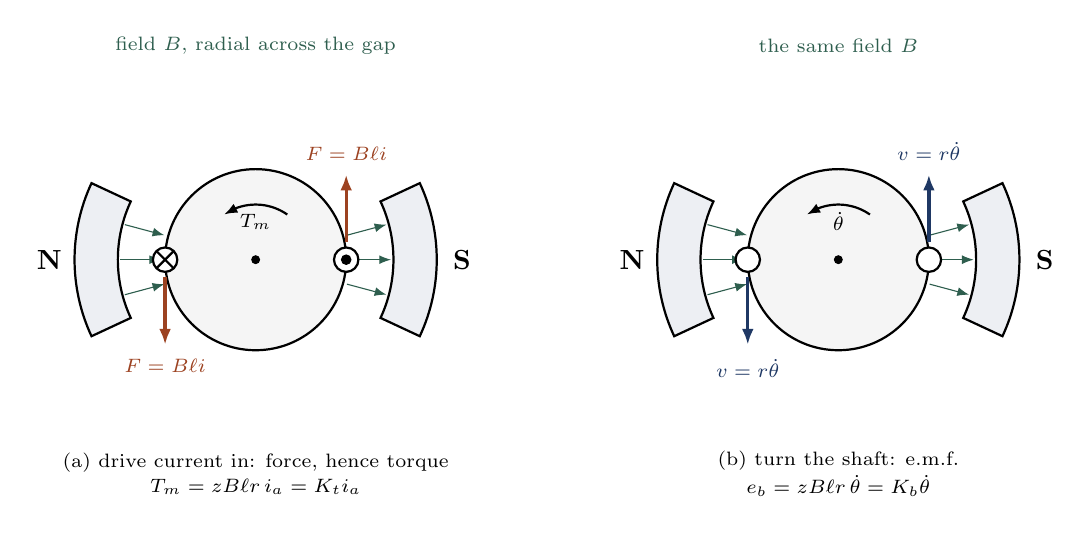
\begin{tikzpicture}[font=\small, x=1cm, y=1cm]
% ---------------- panel (a): motor action ----------------
\begin{scope}
\draw[thick, fill=fnavy!8] (155:1.75) arc (155:205:1.75)
    -- (205:2.30) arc (205:155:2.30) -- cycle;
\draw[thick, fill=fnavy!8] (-25:1.75) arc (-25:25:1.75)
    -- (25:2.30) arc (25:-25:2.30) -- cycle;
\node[font=\bfseries] at (180:2.62) {N};
\node[font=\bfseries] at (0:2.62) {S};
\draw[thick, fill=gray!8] (0,0) circle (1.15);
\draw[fill] (0,0) circle (1.4pt);
\foreach \a in {165,180,195}{\draw[faccent, -{Latex[length=1.5mm]}] (\a:1.72) -- (\a:1.20);}
\foreach \a in {-15,0,15}{\draw[faccent, -{Latex[length=1.5mm]}] (\a:1.20) -- (\a:1.72);}
\node[faccent, font=\scriptsize] at (0,2.72) {field $B$, radial across the gap};
% conductors: current into page (left), out of page (right)
\draw[thick, fill=white] (180:1.15) circle (0.155);
\draw[thick] ($(180:1.15)+(-0.11,-0.11)$) -- ($(180:1.15)+(0.11,0.11)$);
\draw[thick] ($(180:1.15)+(-0.11,0.11)$) -- ($(180:1.15)+(0.11,-0.11)$);
\draw[thick, fill=white] (0:1.15) circle (0.155);
\draw[fill] (0:1.15) circle (1.7pt);
% forces
\draw[fflag, very thick, -{Latex[length=2mm]}] (-1.15,-0.22) -- (-1.15,-1.08);
\node[fflag, font=\scriptsize, anchor=north] at (-1.15,-1.14) {$F=B\ell i$};
\draw[fflag, very thick, -{Latex[length=2mm]}] (1.15,0.22) -- (1.15,1.08);
\node[fflag, font=\scriptsize, anchor=south] at (1.15,1.14) {$F=B\ell i$};
\draw[thick, -{Latex[length=1.7mm]}] (55:0.70) arc (55:125:0.70);
\node[font=\scriptsize] at (90:0.48) {$T_{m}$};
\node[font=\scriptsize, align=center] at (0,-2.72)
  {(a) drive current in: force, hence torque\\[1pt]
   $T_{m}=zB\ell r\,i_{a}=K_{t}i_{a}$};
\end{scope}
% ---------------- panel (b): generator action ----------------
\begin{scope}[shift={(7.4,0)}]
\draw[thick, fill=fnavy!8] (155:1.75) arc (155:205:1.75)
    -- (205:2.30) arc (205:155:2.30) -- cycle;
\draw[thick, fill=fnavy!8] (-25:1.75) arc (-25:25:1.75)
    -- (25:2.30) arc (25:-25:2.30) -- cycle;
\node[font=\bfseries] at (180:2.62) {N};
\node[font=\bfseries] at (0:2.62) {S};
\draw[thick, fill=gray!8] (0,0) circle (1.15);
\draw[fill] (0,0) circle (1.4pt);
\foreach \a in {165,180,195}{\draw[faccent, -{Latex[length=1.5mm]}] (\a:1.72) -- (\a:1.20);}
\foreach \a in {-15,0,15}{\draw[faccent, -{Latex[length=1.5mm]}] (\a:1.20) -- (\a:1.72);}
\node[faccent, font=\scriptsize] at (0,2.72) {the same field $B$};
\draw[thick, fill=white] (180:1.15) circle (0.155);
\draw[thick, fill=white] (0:1.15) circle (0.155);
\draw[fnavy, very thick, -{Latex[length=2mm]}] (-1.15,-0.22) -- (-1.15,-1.08);
\node[fnavy, font=\scriptsize, anchor=north] at (-1.15,-1.14) {$v=r\dot\theta$};
\draw[fnavy, very thick, -{Latex[length=2mm]}] (1.15,0.22) -- (1.15,1.08);
\node[fnavy, font=\scriptsize, anchor=south] at (1.15,1.14) {$v=r\dot\theta$};
\draw[thick, -{Latex[length=1.7mm]}] (55:0.70) arc (55:125:0.70);
\node[font=\scriptsize] at (90:0.48) {$\dot\theta$};
\node[font=\scriptsize, align=center] at (0,-2.72)
  {(b) turn the shaft: e.m.f.\\[1pt]
   $e_{b}=zB\ell r\,\dot\theta=K_{b}\dot\theta$};
\end{scope}
\end{tikzpicture}
\caption{The same conductors, the same field, the same geometry --- read two
ways. Because $zB\ell r$ appears in both \eqref{eq:torqueconst} and
\eqref{eq:emfconst}, $K_{t}$ and $K_{b}$ are not merely similar: in a
consistent set of units they are the \emph{same number}.}
\label{fig:dcmotor}
\end{figure}

% ....................................................................
\subsubsection{Step 3 --- why $K_{t}$ and $K_{b}$ are the same number}

Comparing \eqref{eq:torqueconst} and \eqref{eq:emfconst}, both constants equal
$zB\ell r$. That is suggestive but it depends on an idealised geometry. The
argument that does not is \textbf{conservation of energy}, and it takes two
lines.

The electrical power that disappears from the armature circuit into
electromechanical conversion is the power absorbed by the back e.m.f.,
$P_{\text{elec}}=e_{b}i_{a}$. The mechanical power delivered to the shaft is
$P_{\text{mech}}=T_{m}\dot\theta$. Nothing else happens in between --- copper
loss is already accounted for by $R_{a}i_{a}^{2}$, and stored magnetic energy
does not change in steady state --- so the two are equal:
\[
  e_{b}i_{a}=T_{m}\dot\theta
  \quad\Longrightarrow\quad
  (K_{b}\dot\theta)\,i_{a}=(K_{t}i_{a})\,\dot\theta
  \quad\Longrightarrow\quad
  \boxed{\;K_{t}=K_{b}\;}
\]
after cancelling $i_{a}\dot\theta$, which is legitimate for every operating
point except the trivial one where the motor is doing nothing.

\begin{keyidea}
$K_{t}=K_{b}$ is a statement about \emph{units}, not a coincidence. Check
them: $\si{\newton\metre\per\ampere}=\si{\joule\per\ampere}$ and
$\si{\volt\second\per\radian}=\si{\joule\per\coulomb}\cdot\si{\second}
=\si{\joule\per\ampere}$ (the radian being dimensionless). The two constants
carry the same dimensions because they describe the same energy conversion
seen from opposite ends. This is why a datasheet quoting
$K_{t}=\SI{0.6}{\newton\metre\per\ampere}$ is also telling you
$K_{b}=\SI{0.6}{\volt\second\per\radian}$, and why a question that gives you
one has given you both.
\end{keyidea}

\begin{pitfall}
The equality holds in \textbf{SI}. Datasheets often quote $K_{b}$ in volts per
1000\,rpm and $K_{t}$ in ounce-inches per ampere, and in those units the two
numbers are wildly different --- which leads students to conclude the equality
is false. Convert to \si{\newton\metre\per\ampere} and
\si{\volt\second\per\radian} first, then compare.
\end{pitfall}

% ....................................................................
\subsubsection{Step 4 --- the back e.m.f.\ \emph{is} the motor's damping}
\label{sss:dcdamping}

This is the step that makes the d.c.\ and a.c.\ servomotors one story rather
than two, and it needs no transfer function at all.

Let the shaft turn steadily at $\dot\theta$, so the armature current has
settled and the inductance has nothing to do. Kirchhoff round the armature
circuit gives $v_{a}=R_{a}i_{a}+e_{b}$, hence
$i_{a}=(v_{a}-K_{b}\dot\theta)/R_{a}$, and multiplying by $K_{t}$:

\begin{equation}
  T_{m}=\underbrace{\frac{K_{t}}{R_{a}}\,v_{a}}_{\text{set by the input}}
       \;-\;\underbrace{\frac{K_{t}K_{b}}{R_{a}}\,\dot\theta}_{\text{opposes motion}} .
  \label{eq:dctorquespeed}
\end{equation}

Read \eqref{eq:dctorquespeed} as a family of straight lines: torque against
speed, one line per armature voltage, all with the \emph{same} negative slope
$K_{t}K_{b}/R_{a}$. A torque that grows more negative in proportion to speed is
precisely what viscous friction does. So the back e.m.f.\ contributes an
effective viscous damping coefficient $K_{t}K_{b}/R_{a}$, in parallel with
whatever mechanical friction $b$ the bearings supply.

\begin{figure}[H]
\centering
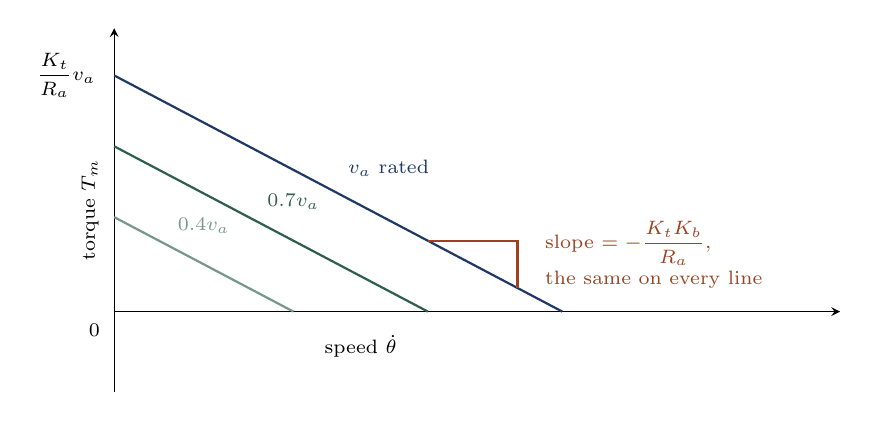
\begin{tikzpicture}
\begin{axis}[
  width=10.8cm, height=6.2cm,
  ylabel={torque $T_{m}$}, ylabel style={font=\scriptsize},
  xmin=0, xmax=1.62, ymin=-0.34, ymax=1.20,
  xtick=\empty, ytick=\empty,
  axis y line=left, axis x line=middle, clip=false,
]
\addplot[fnavy,  thick, domain=0:1.0,  samples=2]{1.0-x};
\addplot[faccent, thick, domain=0:0.7, samples=2]{0.7-x};
\addplot[faccent!65, thick, domain=0:0.4, samples=2]{0.4-x};
\node[fnavy,   font=\scriptsize, anchor=south west] at (axis cs:0.50,0.53) {$v_{a}$ rated};
\node[faccent, font=\scriptsize, anchor=south west] at (axis cs:0.32,0.39) {$0.7v_{a}$};
\node[faccent!65, font=\scriptsize, anchor=south west] at (axis cs:0.12,0.29) {$0.4v_{a}$};
% slope annotation, hung off the rated line
\draw[fflag, thick] (axis cs:0.70,0.30) -- (axis cs:0.90,0.30) -- (axis cs:0.90,0.10);
\node[fflag, font=\scriptsize, anchor=west, align=left] at (axis cs:0.94,0.24)
  {slope $=-\dfrac{K_{t}K_{b}}{R_{a}}$,\\[1pt] the same on every line};
\node[font=\scriptsize, anchor=east] at (axis cs:-0.02,1.0) {$\dfrac{K_{t}}{R_{a}}v_{a}$};
\node[font=\scriptsize, anchor=north east] at (axis cs:-0.01,-0.01) {$0$};
\node[font=\scriptsize, anchor=north] at (axis cs:0.55,-0.06) {speed $\dot\theta$};
\end{axis}
\end{tikzpicture}
\caption{The armature-controlled d.c.\ motor's torque--speed characteristic,
\eqref{eq:dctorquespeed}. Raising the armature voltage lifts the line without
tilting it. The negative slope is the back e.m.f.\ acting as viscous friction;
compare Figure~\ref{fig:acslope}, where an a.c.\ servomotor achieves the same
negative slope by a completely different mechanism.}
\label{fig:dcslope}
\end{figure}

Two things follow immediately, without doing any more algebra.

\begin{itemize}[leftmargin=1.5em,itemsep=2pt]
\item \textbf{A d.c.\ motor is self-damping.} Lower $R_{a}$ and the slope
      steepens: a low-resistance armature is a heavily damped one. Drive the
      same motor from a high-impedance (current) source instead and that
      damping disappears, because the current --- and hence the torque --- no
      longer responds to the back e.m.f.\ at all.
\item \textbf{Stall torque and no-load speed follow from one line.} Setting
      $\dot\theta=0$ gives the stall torque $K_{t}v_{a}/R_{a}$; setting
      $T_{m}=0$ gives the no-load speed $v_{a}/K_{b}$. Those are the two
      numbers a catalogue quotes, and they fix the whole characteristic.
\end{itemize}

% ....................................................................
\subsubsection{The transfer function, and where it is derived}

Add the mechanical equation $T_{m}=J_{m}\ddot\theta_{m}+b\dot\theta_{m}$ and
the armature inductance $L_{a}$, take Laplace transforms and eliminate
$I_{a}(s)$, and the result is
\begin{equation}
  \frac{\theta_{m}(s)}{V_{a}(s)}
     =\frac{K_{t}}{s\big[(R_{a}+L_{a}s)(J_{m}s+b)+K_{t}K_{b}\big]}
     \;\xrightarrow[\;L_{a}\to0\;]{}\;
     \frac{K_{m}}{s(\tau_{m}s+1)},
  \label{eq:dcm}
\end{equation}
\[
  K_{m}=\frac{K_{t}}{R_{a}b+K_{t}K_{b}},
  \qquad
  \tau_{m}=\frac{J_{m}R_{a}}{R_{a}b+K_{t}K_{b}} .
\]
Notice the denominator: $R_{a}b$ is the mechanical friction's contribution and
$K_{t}K_{b}$ is the electromechanical damping of \S\ref{sss:dcdamping},
appearing exactly where \eqref{eq:dctorquespeed} says it should. In most
servomotors $K_{t}K_{b}$ is the larger of the two, so the motor's own back
e.m.f.\ supplies most of its damping.

\statedin{The elimination of $I_{a}(s)$, the effect of keeping $L_{a}$, gear
reflection and worked numbers are the Week~2 lecture and tutorial --- see
\texttt{week-02-notes.pdf} \S6 and \texttt{week-02-tutorial} Q1. They are not
repeated here; what \emph{is} done here is to supply the two constants that
Week~2 takes as given.}

% ....................................................................
\subsubsection{Field control, and why it is slower}
\label{sss:field}

Hold the armature current constant at $I_{a}$ and vary the field instead. Now
$B$ in \eqref{eq:torqueconst} is proportional to the field current $i_{f}$, so
\[
  T_{m}=K_{f}\,i_{f},\qquad
  v_{f}=R_{f}i_{f}+L_{f}\frac{\mathrm{d}i_{f}}{\mathrm{d}t},
\]
and combining these with $T_{m}=J\ddot\theta+b\dot\theta$ gives
\begin{equation}
  \frac{\theta(s)}{V_{f}(s)}
   =\frac{K_{f}}{s\,(R_{f}+L_{f}s)(Js+b)}
   =\frac{K}{s(\tau_{f}s+1)(\tau_{m}s+1)},
  \qquad \tau_{f}=\frac{L_{f}}{R_{f}},\ \ \tau_{m}=\frac{J}{b}.
  \label{eq:fieldctl}
\end{equation}
Compare this with \eqref{eq:dcm} and two differences stand out, both of them
disadvantages.

\begin{itemize}[leftmargin=1.5em,itemsep=2pt]
\item \textbf{There is no $K_{t}K_{b}$ term.} With the armature current forced
      constant, the back e.m.f.\ can no longer alter it, so the
      electromechanical damping of \S\ref{sss:dcdamping} is gone and the motor
      is left with only its bearing friction $b$. The field-controlled motor is
      the more lightly damped machine.
\item \textbf{There is an extra lag $\tau_{f}$.} The field winding is built for
      many turns and low current, so $L_{f}$ is large and $\tau_{f}$ is long.
      The armature circuit it replaced was fast enough that
      \eqref{eq:dcm} routinely throws it away; the field circuit is not.
\end{itemize}

Its one advantage is power: the field carries a small current, so the amplifier
driving it is cheap. Field control survives where that matters more than
speed of response.

\paragraph{The amplidyne.} Before solid-state amplifiers, large d.c.\ systems
were driven by an \textbf{amplidyne} --- a cross-field d.c.\ machine with two
brush sets $90^\circ$ apart, the quadrature pair short-circuited so that the
machine amplifies twice within one frame (power gains of roughly $200$ then
$50$, so about $10^{4}$ overall). It is obsolete, displaced by thyristor and
IGBT drives, but it is all over older textbook problems and worth recognising.
Nagrath \& Gopal \S4.3, p.~90.

% --------------------------------------------------------------------
\subsection{The a.c.\ (two-phase) servomotor}

Preferred at low power, and the natural partner of a synchro error detector
because the signals are already carrier-modulated a.c. It is rugged, light and
brushless. Nagrath \& Gopal \S4.3, pp.~84--88.

% ....................................................................
\subsubsection{The rotating field --- and how it differs from the synchro's}
\label{sss:rotating}

Structurally it is a two-phase induction motor: two stator windings
$90^\circ$ apart \emph{in space}, excited by voltages $90^\circ$ apart \emph{in
time}. Sum the two m.m.f.\ vectors exactly as in \S\ref{sss:rebuild}, putting
winding~1 along $\hat{u}(0)$ and winding~2 along $\hat{u}(90^\circ)$:
\begin{equation}
  \mathbf{F}(t)=F_{m}\cos\omega t\;\hat{u}(0)
              + F_{m}\cos(\omega t-90^\circ)\;\hat{u}(90^\circ)
              = F_{m}\big(\cos\omega t,\;\sin\omega t\big).
  \label{eq:rotfield}
\end{equation}
The magnitude is $F_{m}$ at every instant, and the direction advances at
$\omega$ radians per second. This is a \textbf{rotating field of constant
magnitude}, turning at synchronous speed. It sweeps past the short-circuited
rotor, induces currents in it, and drags it round --- ordinary induction-motor
action.

\begin{keyidea}
The synchro of \S\ref{sec:synchro} and the two-phase motor use the \emph{same}
vector sum over stator coils. The only difference is how the coil currents are
phased in time, and it changes everything:
\begin{center}
\begin{tabular}{lll}
\toprule
 & synchro stator & two-phase motor \\
\midrule
coils          & three, $120^\circ$ apart & two, $90^\circ$ apart \\
amplitudes     & unequal, set by $\theta$ & equal \\
time phase     & all identical            & $90^\circ$ apart \\
resultant      & \emph{stationary}, pulsating & \emph{rotating}, constant magnitude \\
tip traces     & a straight line          & a circle \\
\bottomrule
\end{tabular}
\end{center}
Getting these two confused is the single most common error in this material.
\end{keyidea}

\begin{figure}[H]
\centering
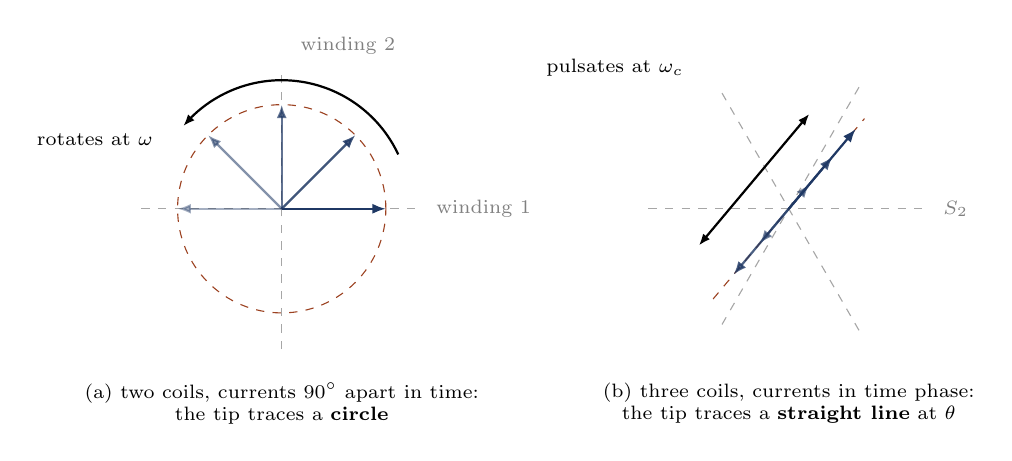
\begin{tikzpicture}[font=\small, x=1.15cm, y=1.15cm]
% ---------------- (a) two-phase: circle locus ----------------
\begin{scope}
\draw[dashed, gray!70] (-1.55,0) -- (1.55,0);
\draw[dashed, gray!70] (0,-1.55) -- (0,1.55);
\node[gray, font=\scriptsize, anchor=west] at (1.6,0) {winding 1};
\node[gray, font=\scriptsize, anchor=south west] at (0.10,1.60) {winding 2};
\draw[fflag, thin, dashed] (0,0) circle (1.15);
\foreach \a/\op in {0/1.0, 45/0.85, 90/0.7, 135/0.55, 180/0.4}{
  \draw[fnavy, thick, opacity=\op, -{Latex[length=1.7mm]}] (0,0) -- (\a:1.15);}
\draw[thick,-{Latex[length=1.5mm]}] (25:1.42) arc (25:140:1.42);
\node[font=\scriptsize, anchor=east] at (150:1.52) {rotates at $\omega$};
\node[font=\scriptsize, align=center] at (0,-2.15)
  {(a) two coils, currents $90^\circ$ apart in time:\\
   the tip traces a \textbf{circle}};
\end{scope}
% ---------------- (b) synchro: line locus ----------------
\begin{scope}[shift={(5.6,0)}]
\foreach \a in {0,120,240}{\draw[dashed, gray!70] (\a-180:1.55) -- (\a:1.55);}
\node[gray, font=\scriptsize, anchor=west] at (1.6,0) {$S_{2}$};
\draw[fflag, thin, dashed] (50-180:1.30) -- (50:1.30);
\foreach \r/\op in {1.15/1.0, 0.75/0.8, 0.35/0.6}{
  \draw[fnavy, thick, opacity=\op, -{Latex[length=1.7mm]}] (0,0) -- (50:\r);}
\foreach \r/\op in {0.5/0.6, 0.95/0.8}{
  \draw[fnavy, thick, opacity=\op, -{Latex[length=1.7mm]}] (0,0) -- (230:\r);}
\draw[thick,{Latex[length=1.5mm]}-{Latex[length=1.5mm]}]
   ($(140:0.50)+(50:0.95)$) -- ($(140:0.50)+(230:0.95)$);
\node[font=\scriptsize, anchor=south east] at (128:1.72) {pulsates at $\omega_{c}$};
\node[font=\scriptsize, align=center] at (0,-2.15)
  {(b) three coils, currents in time phase:\\
   the tip traces a \textbf{straight line} at $\theta$};
\end{scope}
\end{tikzpicture}
\caption{The same vector sum, two different time phasings. In (a) the coil
currents are in time quadrature and the resultant sweeps round at constant
length; in (b) --- the synchro of \S\ref{sec:synchro} --- they are in time
phase, and the resultant stands still along the direction $\theta$ while its
length pulsates through zero and reverses.}
\label{fig:loci}
\end{figure}

\paragraph{Reversing it.} Feed the control phase at $+90^\circ$ instead of
$-90^\circ$ and \eqref{eq:rotfield} becomes
\[
  \mathbf{F}(t)=F_{m}\big(\cos\omega t,\;-\sin\omega t\big):
\]
same constant magnitude, opposite direction of rotation. That is the entire
steering mechanism of the machine.
The \emph{reference phase} is held at a fixed voltage, the \emph{control
phase} is driven by the servo amplifier, and the \emph{sign} of the control
signal --- carried, as \S\ref{sss:carrier} showed, in the phase of the carrier
--- decides which way the shaft turns. The error detector's phase information
is consumed here, by the motor itself.

% ....................................................................
\subsubsection{Why the rotor must have a \emph{high} resistance}
\label{sss:highR}

Every ordinary induction motor is designed with rotor resistance as low as
practicable, to keep the rotor copper loss down. The servomotor deliberately
does the opposite. The reason is visible in the torque--slip relation.

For an induction machine with rotor resistance $R$ and standstill rotor
reactance $X$, running at slip $s$, the standard approximate torque (neglecting
stator impedance) is
\begin{equation}
  T\;\propto\;\frac{s\,R}{R^{2}+s^{2}X^{2}} .
  \label{eq:torqueslip}
\end{equation}
Differentiate and set to zero: the maximum occurs at
\begin{equation}
  s_{\max}=\frac{R}{X},
  \qquad\text{and there}\qquad
  T_{\max}\propto\frac{1}{2X}
  \quad\text{--- independent of }R.
  \label{eq:smax}
\end{equation}
Raising the rotor resistance does not change how much torque the machine can
produce; it changes \emph{where} that maximum sits. And since slip runs from
$s=1$ at standstill down to $s=0$ at synchronous speed, everything turns on
whether $s_{\max}$ falls inside that interval:

\begin{itemize}[leftmargin=1.5em,itemsep=3pt]
\item \textbf{Ordinary motor, $X/R$ large.} Then $s_{\max}=R/X$ is small ---
      typically a few per cent --- so the peak sits close to synchronous speed.
      Over the whole range from standstill up to $s_{\max}$, torque
      \emph{rises} as the motor speeds up. That is a \textbf{positive}
      torque--speed slope.
\item \textbf{Servomotor, $R\ge X$.} Then $s_{\max}\ge1$, so the peak lies at
      or beyond standstill and is never reached in normal running. Over the
      entire operating range torque falls monotonically as speed rises: the
      slope is \textbf{negative everywhere}.
\end{itemize}

There is a bonus. When $R\gg sX$ the denominator of \eqref{eq:torqueslip} is
dominated by $R^{2}$ and $T\propto s/R$ --- torque becomes very nearly
\emph{linear} in slip, and therefore linear in speed. So the one design
change buys both properties the control engineer needs: a negative slope, and
a straight enough line to linearise about.

\begin{figure}[H]
\centering
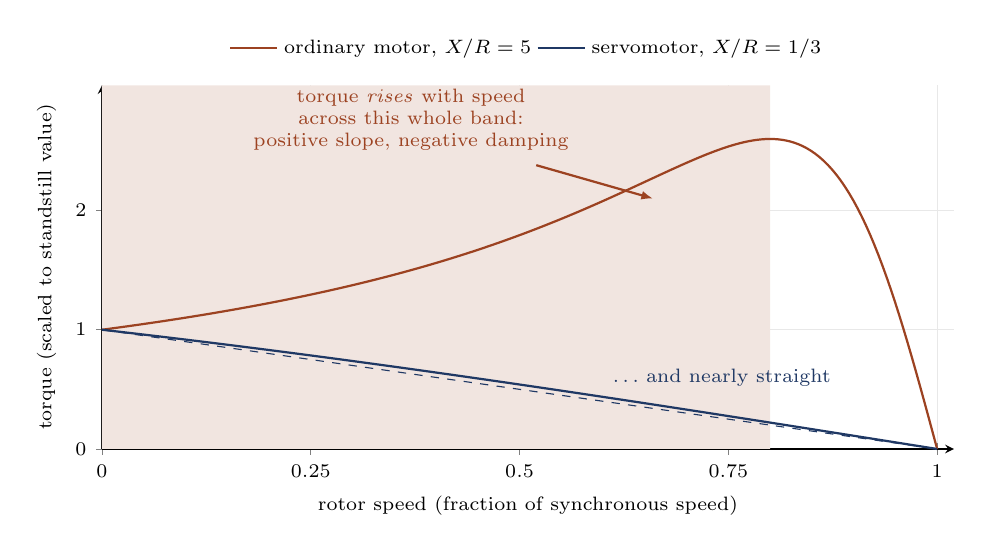
\begin{tikzpicture}
\begin{axis}[
  width=12.4cm, height=6.2cm,
  xlabel={rotor speed (fraction of synchronous speed)},
  ylabel={torque (scaled to standstill value)},
  xlabel style={font=\scriptsize}, ylabel style={font=\scriptsize},
  xmin=0, xmax=1.02, ymin=0, ymax=3.05,
  xtick={0,0.25,0.5,0.75,1}, ytick={0,1,2},
  tick label style={font=\scriptsize},
  grid=both, grid style={gray!18},
  axis lines=left, clip=false,
  legend style={font=\scriptsize, at={(0.5,1.16)}, anchor=north,
                legend columns=2, draw=none},
]
% the speed range over which the ordinary motor's slope is positive
\addplot[draw=none, fill=fflag!14, forget plot] coordinates
   {(0,0) (0.8,0) (0.8,3.05) (0,3.05)} \closedcycle;
\addplot[thick, fflag, domain=0:1, samples=200]
   {(1-x)*0.2/(0.04+(1-x)^2)/0.192308};
\addlegendentry{ordinary motor, $X/R=5$}
\addplot[thick, fnavy, domain=0:1, samples=200]
   {(1-x)*3/(9+(1-x)^2)/0.3};
\addlegendentry{servomotor, $X/R=1/3$}
\addplot[thin, fnavy, dashed, domain=0:1, samples=2] {1-x};
\node[fnavy, font=\scriptsize, anchor=south west] at (axis cs:0.60,0.44)
   {\ldots\,and nearly straight};
\node[fflag, font=\scriptsize, anchor=south, align=center] at (axis cs:0.37,2.42)
   {torque \emph{rises} with speed\\across this whole band:\\positive slope, negative damping};
\draw[fflag, thick, -{Latex[length=1.5mm]}] (axis cs:0.52,2.38) -- (axis cs:0.66,2.10);
\end{axis}
\end{tikzpicture}
\caption{Equation~\eqref{eq:torqueslip} plotted for the two designs. The
ordinary motor's peak sits at $s_{\max}=R/X=0.2$, i.e.\ at 80\% of synchronous
speed, leaving the shaded region below it with a positive torque--speed slope.
The servomotor's peak is pushed out to $s_{\max}=3$, beyond standstill, so its
whole characteristic falls --- and it hugs the dashed straight line to within
about 8\%. Cf.\ Nagrath \& Gopal Fig.~4.4, p.~85.}
\label{fig:acslope}
\end{figure}

\begin{pitfall}
A positive torque--speed slope is not merely inconvenient, it is
\emph{destabilising}. As \eqref{eq:acm} below shows, the slope enters the model
as a viscous friction $f$ added to the load's own $f_{0}$. A positive slope
makes $f$ negative, and if it outweighs $f_{0}$ the total damping goes
negative --- the $s$ coefficient of a second-order denominator changes sign,
and the closed loop is unstable. The choice of rotor resistance, apparently a
machine-design detail, reaches all the way into the stability of the control
system.
\end{pitfall}

% ....................................................................
\subsubsection{Linearising the characteristic}

The curves of Figure~\ref{fig:acslope} are still not exactly straight, and
their spacing with control voltage is not exactly uniform. But a servomotor in
a position loop spends its life near zero speed and near zero control voltage,
so linearise there. Torque depends on two variables, speed and the rms control
voltage: $T_{m}=f(\dot\theta,E)$. Expand in a Taylor series about the operating
point $(\dot\theta_{0},E_{0})$ and keep first-order terms:
\[
  T_{m}=T_{m0}
    +\left.\frac{\partial T_{m}}{\partial E}\right|_{0}(E-E_{0})
    +\left.\frac{\partial T_{m}}{\partial\dot\theta}\right|_{0}
      (\dot\theta-\dot\theta_{0}),
\]
which in incremental notation is
\begin{equation}
  \Delta T_{m}=K\,\Delta E-f\,\Delta\dot\theta,
  \qquad
  K=\left.\frac{\partial T_{m}}{\partial E}\right|_{0},
  \qquad
  f=-\left.\frac{\partial T_{m}}{\partial\dot\theta}\right|_{0}.
  \label{eq:aclin}
\end{equation}
The minus sign in the definition of $f$ is deliberate: the slope
$\partial T_{m}/\partial\dot\theta$ is negative, so defining $f$ as its
negative makes $f$ a positive number, and \eqref{eq:aclin} then reads as
``driving torque minus a friction torque''.

With a load of inertia $J$ and friction $f_{0}$, the torque balance is
$\Delta T_{m}=J\Delta\ddot\theta+f_{0}\Delta\dot\theta$. Substituting
\eqref{eq:aclin}, taking Laplace transforms and rearranging:
\begin{equation}
  G_{m}(s)=\frac{\Delta\theta(s)}{\Delta E(s)}
   =\frac{K}{Js^{2}+(f_{0}+f)s}
   =\frac{K_{m}}{s(\tau_{m}s+1)},
  \qquad
  K_{m}=\frac{K}{f_{0}+f},\quad
  \tau_{m}=\frac{J}{f_{0}+f} .
  \label{eq:acm}
\end{equation}
In a position control system the operating point is $(\dot\theta_{0}=0,
E_{0}=0)$, so the increments are the quantities themselves and the $\Delta$s
can be dropped.

\paragraph{Getting $K$ and $f$ from two tests.} The characteristic is fixed by
two standard measurements at rated control voltage: the \textbf{stall torque}
(rotor clamped, $\dot\theta=0$) and the \textbf{no-load speed} ($T_{m}=0$). The
straight line joining them is the working approximation, so
\[
  K\approx\frac{\text{stall torque at rated voltage}}
               {\text{rated control-phase voltage}},
\]
\[
  f\approx\frac{\text{stall torque at rated voltage}}
               {\text{no-load speed at rated voltage}} .
\]
Nagrath adds a practical correction (\S4.3, eq.~4.7, p.~88): in real
servomotors the slope at low speed is nearer \emph{half} the slope of that
joining line, so for position-control work take
$f\approx\tfrac{1}{2}\times(\text{stall torque}/\text{no-load speed})$.

% ....................................................................
\subsubsection{The two motors are the same story}
\label{sss:samething}

\begin{keyidea}
Compare \eqref{eq:dctorquespeed} with \eqref{eq:aclin}. Both say
\emph{developed torque $=$ (a constant) $\times$ (the input) $-$ (a constant)
$\times$ (speed)}, and in both the second constant is a viscous damping that
the machine supplies to itself:
\begin{center}
\begin{tabular}{lll}
\toprule
 & d.c.\ servomotor & a.c.\ servomotor \\
\midrule
input          & armature voltage $v_{a}$ & control-phase voltage $E$ \\
drive constant & $K_{t}/R_{a}$            & $K=\partial T_{m}/\partial E$ \\
damping        & $K_{t}K_{b}/R_{a}$       & $f=-\partial T_{m}/\partial\dot\theta$ \\
its origin     & back e.m.f.              & negative torque--speed slope \\
result         & $K_{m}/[s(\tau_{m}s+1)]$ & $K_{m}/[s(\tau_{m}s+1)]$ \\
\bottomrule
\end{tabular}
\end{center}
Two quite different machines arrive at the same transfer function because both
are governed by the same balance: a driving torque proportional to the input,
opposed by a resisting torque proportional to speed, working against inertia.
The integrator comes from the fact that we want \emph{position} out of a device
that naturally produces \emph{speed}. This is the shape the last section of the
Week~1 notes is about.
\end{keyidea}

% --------------------------------------------------------------------
\subsection{The stepper motor}

A \textbf{stepper motor} converts a train of pulses into a train of discrete
angular steps --- one step per pulse. It is the actuator of incremental motion
control: printers, tape and capstan drives, machine tools, plotters, 3-D
printers. The common types are \emph{variable reluctance} and \emph{permanent
magnet}; what follows is the variable-reluctance machine. Nagrath \& Gopal
\S4.4, pp.~99--103.

The machine has $n$ stacks of stator and rotor on a common frame and shaft,
both toothed with $T$ teeth of the same size. The stators are pulse-excited;
the rotors carry no winding at all. Energise a stator stack and the rotor is
pulled to the nearest \textbf{minimum-reluctance} position --- the one where
its teeth line up with that stack's teeth.

% ....................................................................
\subsubsection{Where the step angle comes from}

The rotor teeth are aligned across every stack, so the rotor by itself has a
single tooth pitch
\[
  \lambda=\frac{360^\circ}{T} .
\]
If the stator stacks were also aligned with one another, energising any of them
would pull the rotor to the same place and the machine could not step at all.
So the stacks are built with their stator teeth offset successively by
$\lambda/n$ --- one $n$-th of a tooth pitch. Energise the next stack in the
sequence and the nearest minimum-reluctance position is now one such offset
away, so the rotor advances by exactly that much:
\begin{equation}
  \alpha=\frac{\lambda}{n}=\frac{360^\circ}{n\,T} .
  \label{eq:step}
\end{equation}
For $n=3$ stacks and $T=12$ teeth, $\alpha=360/36=\SI{10}{\degree}$: thirty-six
pulses per revolution. Note what \eqref{eq:step} says about resolution --- to
make the steps finer you may either add teeth or add stacks, and adding teeth
is by far the cheaper of the two.

\begin{figure}[H]
\centering
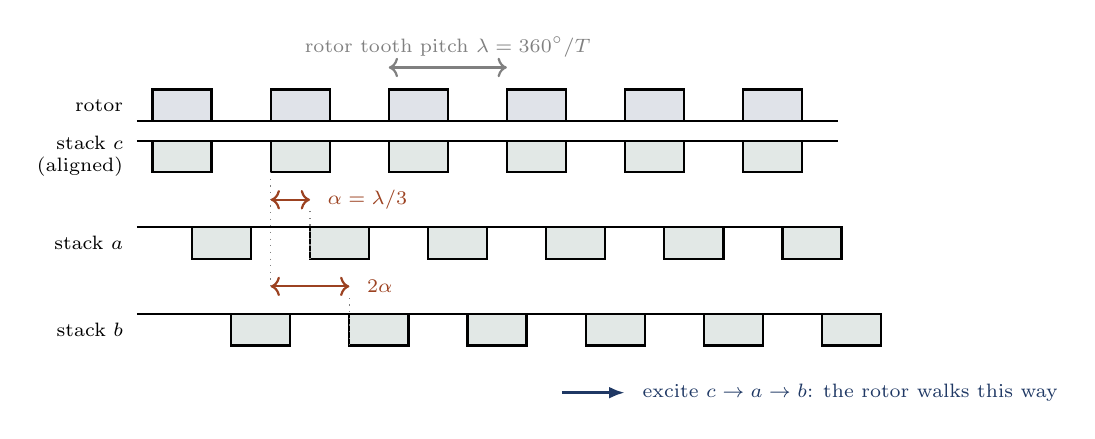
\begin{tikzpicture}[font=\small, x=1cm, y=1cm]
% ---- rotor: teeth aligned across every stack ----
\foreach \i in {0,...,5}{
  \draw[thick,fill=fnavy!14] ({\i*1.5},3.10) rectangle ({\i*1.5+0.75},3.50);}
\draw[thick] (-0.2,3.10) -- (8.7,3.10);
\node[left, font=\scriptsize] at (-0.25,3.30) {rotor};
% ---- stack c: aligned with the rotor ----
\foreach \i in {0,...,5}{
  \draw[thick,fill=faccent!14] ({\i*1.5},2.45) rectangle ({\i*1.5+0.75},2.85);}
\draw[thick] (-0.2,2.85) -- (8.7,2.85);
\node[left, font=\scriptsize, align=right] at (-0.25,2.65) {stack $c$\\(aligned)};
% ---- stack a: offset by one third of a pitch ----
\foreach \i in {0,...,5}{
  \draw[thick,fill=faccent!14] ({\i*1.5+0.5},1.35) rectangle ({\i*1.5+1.25},1.75);}
\draw[thick] (-0.2,1.75) -- (8.7,1.75);
\node[left, font=\scriptsize] at (-0.25,1.55) {stack $a$};
% ---- stack b: offset by two thirds ----
\foreach \i in {0,...,5}{
  \draw[thick,fill=faccent!14] ({\i*1.5+1.0},0.25) rectangle ({\i*1.5+1.75},0.65);}
\draw[thick] (-0.2,0.65) -- (8.7,0.65);
\node[left, font=\scriptsize] at (-0.25,0.45) {stack $b$};
% ---- the two offsets ----
\draw[dotted, gray] (1.5,2.45) -- (1.5,0.95);
\draw[dotted, gray] (2.0,1.35) -- (2.0,2.02);
\draw[dotted, gray] (2.5,0.25) -- (2.5,0.92);
\draw[<->, thick, fflag] (1.5,2.10) -- (2.0,2.10);
\node[fflag, font=\scriptsize, anchor=west] at (2.10,2.10) {$\alpha=\lambda/3$};
\draw[<->, thick, fflag] (1.5,1.00) -- (2.5,1.00);
\node[fflag, font=\scriptsize, anchor=west] at (2.60,1.00) {$2\alpha$};
% ---- rotor tooth pitch ----
\draw[<->, thick, gray] (3.0,3.78) -- (4.5,3.78);
\node[gray, font=\scriptsize, above] at (3.75,3.79)
   {rotor tooth pitch $\lambda=360^\circ/T$};
% ---- excitation sequence ----
\draw[fnavy, very thick, -{Latex[length=2mm]}] (5.2,-0.35) -- (6.0,-0.35);
\node[fnavy, font=\scriptsize, anchor=west] at (6.1,-0.35)
   {excite $c\to a\to b$: the rotor walks this way};
\end{tikzpicture}
\caption{Developed (rolled-out) view of a three-stack variable-reluctance
stepper. The rotor teeth line up across all three stacks; the stator stacks are
offset from one another by a third of a tooth pitch. Energising $c$, then $a$,
then $b$ walks the rotor forward one $\alpha$ at a time. Cf.\ Nagrath \& Gopal
Figs.~4.18 and 4.20, pp.~100--101.}
\label{fig:stepper}
\end{figure}

% ....................................................................
\subsubsection{Where the torque comes from}

The rotor carries no current, so there is no $B\ell i$ force to appeal to. The
torque is a \textbf{reluctance} torque, and it comes from the fact that the
stator winding's inductance depends on where the rotor is.

Assume the magnetic circuit is linear, so $L$ depends on rotor position only.
The energy stored in the field is
\[
  W=\tfrac{1}{2}L(\theta)\,i^{2},
\]
and the torque is the rate at which that stored energy changes with position at
constant current,
\begin{equation}
  T_{m}=\frac{\partial W}{\partial\theta}\bigg|_{i}
       =\tfrac{1}{2}\,i^{2}\,\frac{\mathrm{d}L}{\mathrm{d}\theta} .
  \label{eq:reluctorque}
\end{equation}
Read that: \emph{the rotor moves so as to increase the inductance}, which is
the same thing as decreasing the reluctance --- the qualitative rule stated
above, now with a formula behind it.

For a toothed structure the inductance is a maximum when teeth align, a minimum
a half-pitch away, and smooth in between, so it is an even, periodic function
of $\theta$ with period $\lambda=360^\circ/T$:
\[
  L(\theta)=L_{1}+L_{2}\cos T\theta .
\]
Substituting into \eqref{eq:reluctorque},
\begin{equation}
  T_{m}=-\tfrac{1}{2}L_{2}T\,i^{2}(t)\,\sin T\theta
       =-K\,i^{2}(t)\,\sin T\theta .
  \label{eq:steptorque}
\end{equation}

\begin{figure}[H]
\centering
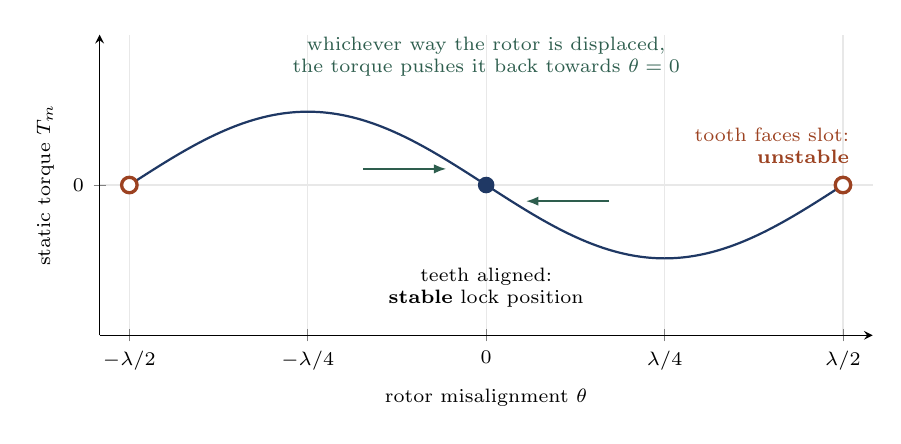
\begin{tikzpicture}
\begin{axis}[
  width=11.4cm, height=5.4cm,
  xlabel={rotor misalignment $\theta$},
  ylabel={static torque $T_{m}$},
  xlabel style={font=\scriptsize}, ylabel style={font=\scriptsize},
  domain=-180:180, samples=241,
  xmin=-195, xmax=195, ymin=-2.05, ymax=2.05,
  xtick={-180,-90,0,90,180},
  xticklabels={$-\lambda/2$,$-\lambda/4$,$0$,$\lambda/4$,$\lambda/2$},
  ytick={0},
  tick label style={font=\scriptsize},
  grid=both, grid style={gray!18},
  axis lines=left, clip=false,
]
\addplot[thick, fnavy] {-sin(x)};
\draw[fnavy, fill=fnavy] (axis cs:0,0) circle (2.8pt);
\draw[fflag, very thick, fill=white] (axis cs:180,0) circle (2.8pt);
\draw[fflag, very thick, fill=white] (axis cs:-180,0) circle (2.8pt);
\draw[faccent, thick, -{Latex[length=1.6mm]}] (axis cs:62,-0.22) -- (axis cs:20,-0.22);
\draw[faccent, thick, -{Latex[length=1.6mm]}] (axis cs:-62,0.22) -- (axis cs:-20,0.22);
\node[font=\scriptsize, anchor=north, align=center] at (axis cs:0,-1.00)
   {teeth aligned:\\\textbf{stable} lock position};
\node[fflag, font=\scriptsize, anchor=south east, align=right] at (axis cs:188,0.16)
   {tooth faces slot:\\\textbf{unstable}};
\node[font=\scriptsize, faccent, anchor=south, align=center] at (axis cs:0,1.35)
   {whichever way the rotor is displaced,\\the torque pushes it back towards $\theta=0$};
\end{axis}
\end{tikzpicture}
\caption{The static torque--angle curve \eqref{eq:steptorque} of one stack, for
a fixed excitation current. The aligned position is stable --- displace the
rotor either way and the torque drives it back. The tooth-faces-slot position a
half-pitch away is an equilibrium too, but an unstable one: any disturbance
sends the rotor off to one of the neighbouring stable positions. Cf.\ Nagrath
\& Gopal Fig.~4.19, p.~101.}
\label{fig:steptorque}
\end{figure}

\paragraph{Why three phases are the minimum.} Directional control needs a pulse
sequence that is different read forwards and backwards. With three stacks,
$abcabc\ldots$ advances the rotor and $bacbac\ldots$ reverses it --- two
distinct sequences. With two, $ababab\ldots$ read backwards is
$bababa\ldots$, which is the same cyclic sequence, so there is nothing to
distinguish one direction from the other. \emph{Directional control requires
three or more phases.}

% ....................................................................
\subsubsection{Why the stepper is not in the analysis weeks}

Equation~\eqref{eq:steptorque} contains $i^{2}$ and $\sin T\theta$: it is
nonlinear in the current \emph{and} in the position, and no linearisation of it
is useful over a whole step. Worse, the stator circuit equation itself carries
a speed term,
\[
  e(t)=Ri+\frac{\mathrm{d}}{\mathrm{d}t}\big[L(\theta)i\big]
      =\underbrace{Ri+L(\theta)\frac{\mathrm{d}i}{\mathrm{d}t}}_{\text{transformer e.m.f.}}
       +\underbrace{i\frac{\mathrm{d}L}{\mathrm{d}\theta}\dot\theta}_{\text{speed e.m.f.}},
\]
which multiplies two unknowns together. Stepper dynamics are solved
numerically, and that is why the machine, useful as it is, does not appear in
the analysis weeks of this unit.

Two consequences do matter for control, though.

\begin{itemize}[leftmargin=1.5em,itemsep=2pt]
\item \textbf{The stepper is a digital actuator.} Shaft position is determined
      entirely by the pulse count, so an \emph{open-loop} step servo can reach
      the accuracy of a closed-loop analogue system with no position sensor at
      all. This is the rare case where open loop is the right engineering
      answer, and it is worth holding on to as a counterexample to the general
      argument for feedback.
\item \textbf{The price is skipped steps.} If pulses arrive faster than the
      rotor can settle into its lock position, or if it overshoots too far,
      a step is lost --- and because nothing is measured, it is lost silently
      and permanently, and every subsequent position is wrong by $\alpha$.
      High-performance systems therefore close the loop after all, gating the
      pulse train from a position feedback signal.
\end{itemize}

% ====================================================================
\section{Sensors: the tachogenerator}
\label{sec:tacho}

A \textbf{tachogenerator} produces a voltage proportional to shaft speed:
\begin{equation}
  v_{t}=K_{t}\,\dot\theta,
  \qquad [K_{t}]=\si{\volt\second\per\radian}.
  \label{eq:tacho}
\end{equation}
It is the only sensor Part~B treats in its own right, and it earns that place
because of what is done with it, which is the subject of \S\ref{sss:ratefb}.

\begin{pitfall}
The symbol $K_{t}$ now means two different things. In \S\ref{sec:actuators} it
was the d.c.\ motor's \emph{torque} constant, in \si{\newton\metre\per\ampere};
here it is the \emph{tachometer} constant, in \si{\volt\second\per\radian}.
This clash is in Nagrath and in most of the literature, so it is not worth
inventing private notation to avoid --- but read the units, not the letter.
Confusingly, the tachometer constant has the same units as the motor's
back-e.m.f.\ constant $K_{b}$, and for good reason: \S\ref{sec:tacho} is about
to show that it is the same quantity.
\end{pitfall}

% --------------------------------------------------------------------
\subsection{The d.c.\ tachogenerator: an equation you have already derived}

A d.c.\ tachogenerator is a small permanent-magnet d.c.\ generator on the
shaft. Its governing equation is \eqref{eq:emfconst} --- the back-e.m.f.\
relation of \S\ref{sss:emfconst}, with nothing changed but the name:
\[
  e_{b}=K_{b}\dot\theta
  \qquad\text{becomes}\qquad
  v_{t}=K_{t}\dot\theta .
\]
There is no new physics here whatever. Every d.c.\ motor already generates a
voltage proportional to its speed; the trouble is that it appears inside the
armature circuit, in series with $R_{a}i_{a}$, where it cannot be measured
without also measuring the current. A tachogenerator is simply that same
conductors-cutting-flux effect given its own machine and its own terminals, so
the speed signal comes out where an amplifier can use it. Its polarity follows
the direction of rotation, so the sign of the speed survives. Its main
limitation is ripple from commutation.

% --------------------------------------------------------------------
\subsection{The a.c.\ (drag-cup) tachogenerator}

Where the loop is a carrier system, the tachometer must produce a
carrier-modulated signal like everything else. The drag-cup tachometer does
this, and it is worth following through because it is the third device in these
notes built out of the same two ideas --- coils in space quadrature, and a
flux whose coupling depends on motion.

Two stator coils sit at right angles: a \textbf{reference} coil, excited from
the carrier supply, and a \textbf{quadrature} coil, from which the output is
taken. The rotor is a thin aluminium cup spinning in the air gap --- a
short-circuited secondary of very low inertia. With the shaft standing still,
the two coils are in space quadrature and there is no coupling between them:
the reference flux threads the quadrature coil edge-on and induces nothing.
Rotation is what breaks that symmetry.

\begin{figure}[H]
\centering
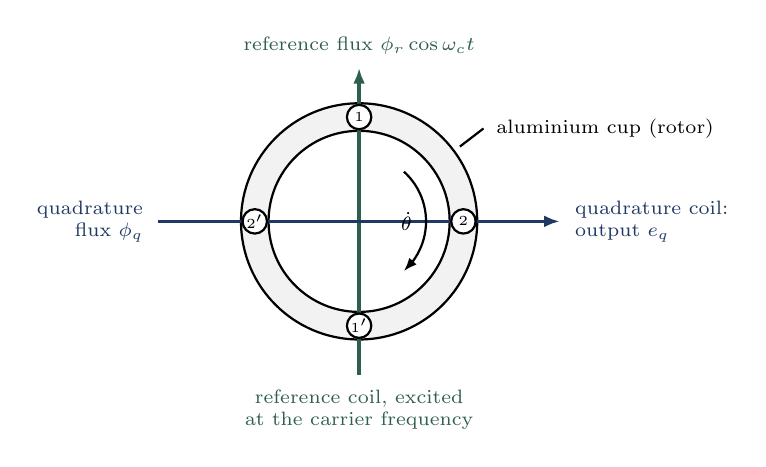
\begin{tikzpicture}[font=\small, x=1cm, y=1cm]
% cup
\draw[thick, fill=gray!10] (0,0) circle (1.5);
\draw[thick, fill=white] (0,0) circle (1.15);
\node[font=\scriptsize, anchor=west] at (1.62,1.18) {aluminium cup (rotor)};
\draw[thick] (1.28,0.95) -- (1.58,1.18);
% reference axis (vertical)
\draw[faccent, very thick, -{Latex[length=2mm]}] (0,-1.95) -- (0,1.95);
\node[faccent, font=\scriptsize, anchor=south, align=center] at (0,2.0)
   {reference flux $\phi_{r}\cos\omega_{c}t$};
\node[faccent, font=\scriptsize, anchor=north, align=center] at (0,-2.02)
   {reference coil, excited\\at the carrier frequency};
% quadrature axis (horizontal)
\draw[fnavy, very thick, -{Latex[length=2mm]}] (-2.55,0) -- (2.55,0);
\node[fnavy, font=\scriptsize, anchor=west, align=left] at (2.62,0)
   {quadrature coil:\\output $e_{q}$};
\node[fnavy, font=\scriptsize, anchor=east, align=right] at (-2.62,0)
   {quadrature\\flux $\phi_{q}$};
% imaginary conductor pairs: (1,1') sit ON the reference axis, where the
% radial field is strongest; a current in them has its magnetic axis at 90 deg,
% i.e. along the quadrature axis.
\draw[fill=white, thick] (0,1.325) circle (0.155);  \node[font=\tiny] at (0,1.325) {$1$};
\draw[fill=white, thick] (0,-1.325) circle (0.155); \node[font=\tiny] at (0,-1.325) {$1'$};
\draw[fill=white, thick] (1.325,0) circle (0.155);  \node[font=\tiny] at (1.325,0) {$2$};
\draw[fill=white, thick] (-1.325,0) circle (0.155); \node[font=\tiny] at (-1.325,0) {$2'$};
% rotation
\draw[thick, -{Latex[length=1.7mm]}] (48:0.85) arc (48:-48:0.85);
\node[font=\scriptsize, anchor=west] at (0.95,0) {};
\node[font=\scriptsize] at (0:0.60) {$\dot\theta$};
\end{tikzpicture}
\caption{The a.c.\ (drag-cup) tachometer. The cup is treated as two imaginary
short-circuited conductor pairs. Pair $(1,1')$ sits \emph{on} the reference
axis, where the radial field is strongest, so it develops the largest speed
voltage --- and because a current loop's magnetic axis is perpendicular to the
line joining its two sides, the current it drives produces a flux along the
\emph{quadrature} axis, which is exactly what the output coil sees.
Cf.\ Nagrath \& Gopal Fig.~4.7, p.~88.}
\label{fig:actacho}
\end{figure}

The chain has four links, and each is one line.

\begin{enumerate}[leftmargin=2em,itemsep=3pt]
\item \textbf{Reference flux.} The reference coil is driven from the carrier
      supply, $v_{r}=V_{r}\sin\omega_{c}t$. Since its resistance and leakage
      are small, essentially all of that voltage is absorbed by
      $N\,\mathrm{d}\phi/\mathrm{d}t$, so the flux \emph{lags the voltage by
      $90^\circ$}: write it $\phi_{r}\cos\omega_{c}t$, pulsating along the
      reference axis.
\item \textbf{Speed voltage in the cup.} Treat the cup as two imaginary
      short-circuited conductor pairs: $(1,1')$ sitting on the reference axis
      and $(2,2')$ a quarter-turn from it. The field crossing the gap is
      strongest --- and most nearly radial --- where it faces the reference
      axis, so it is pair $(1,1')$ that cuts the most flux as the cup turns.
      By the same $B\ell v$ law as \S\ref{sss:emfconst}, its speed voltage is
      proportional to the \emph{product} of flux and speed:
      \[
        e_{1}\;\propto\;\big(\phi_{r}\cos\omega_{c}t\big)\,\dot\theta(t).
      \]
\item \textbf{Quadrature flux.} The cup is short-circuited, so that voltage
      drives a current; with the cup's reactance negligible the current is in
      phase with it. Now comes the geometric step: a current loop's magnetic
      axis is \emph{perpendicular} to the line joining its two sides, so a
      current in $(1,1')$ --- which lie on the reference axis --- produces a
      flux along the \textbf{quadrature} axis:
      \[
        \phi_{q}\;\propto\;\dot\theta(t)\,\cos\omega_{c}t .
      \]
      This is why the output coil has to be at right angles to the reference
      coil. At standstill the two are magnetically decoupled and the output is
      zero; rotation is the only thing that creates a flux along the axis the
      output coil can see.
\item \textbf{Output.} The quadrature coil sees $\phi_{q}$ and responds to its
      rate of change:
      \[
        e_{q}\propto\frac{\mathrm{d}\phi_{q}}{\mathrm{d}t}
        \propto\underbrace{\ddot\theta\,\cos\omega_{c}t}_{\text{small}}
              -\underbrace{\omega_{c}\,\dot\theta\sin\omega_{c}t}_{\text{dominant}} .
      \]
      If the shaft speed varies slowly compared with the carrier --- the same
      condition as in \S\ref{sss:carrier} --- the first term is negligible
      against the second, and, absorbing the sign into the sense of the output
      winding,
      \begin{equation}
        e_{q}(t)=K_{t}\,\dot\theta(t)\,\sin\omega_{c}t .
        \label{eq:actacho}
      \end{equation}
\end{enumerate}

Note what happened to the phase along the way: the reference winding put the
flux $90^\circ$ behind its excitation, and the output winding, by
differentiating, put that $90^\circ$ straight back. The two cancel, so
$e_{q}$ comes out \emph{in phase with the carrier supply} --- exactly like the
synchro's output \eqref{eq:linear}. That is not an accident of algebra but the
reason the two devices can be summed in the same loop at all: fed from one
carrier, their signals are commensurate, and the amplifier can add them
without any phase-shifting network between.

So the a.c.\ tachometer, like the synchro pair, delivers a
\textbf{suppressed-carrier} signal: amplitude proportional to speed, phase
reversing with direction, and nothing at all at the output when the shaft is
still. It plugs straight into a carrier loop without a demodulator, which is
the point of building it this way. Its very low rotor inertia is the other
advantage --- a sensor that loads the shaft it is measuring is a poor sensor.

% --------------------------------------------------------------------
\subsection{What a tachometer is \emph{for}}
\label{sss:ratefb}

Tachometers are used in two quite different ways, and it is worth separating
them.

\begin{enumerate}[leftmargin=2em,itemsep=2pt]
\item As the \textbf{sensor of a speed control loop}, where speed is the
      controlled variable. Unremarkable: it is the feedback element, doing what
      the potentiometer does in a position loop.
\item As \textbf{rate feedback} inside a \emph{position} loop, where the
      tachometer signal is fed back through an inner loop that the outer
      position loop knows nothing about. This is the interesting one, and it is
      the first compensator you meet in this unit.
\end{enumerate}

Take Nagrath's a.c.\ position control system (\S4.3, p.~96): synchro pair of
sensitivity $K_{s}$, amplifier $K_{a}$, a.c.\ servomotor
$K_{m}/[s(\tau_{m}s+1)]$, gearing $n$, and a tachometer of constant $K_{t}$
feeding back around the motor. Work inwards. The inner loop, from amplifier
input $u$ to motor shaft $\theta_{m}$, closes to
\[
  \frac{\theta_{m}}{u}
   =\frac{K_{a}K_{m}}{s(\tau_{m}s+1)+K_{a}K_{m}K_{t}s}
   =\frac{K_{a}K_{m}}{s\big(\tau_{m}s+1+K_{a}K_{m}K_{t}\big)} ,
\]
and closing the outer loop around that, with $\theta_{c}=n\theta_{m}$ and
$u=K_{s}(\theta_{r}-\theta_{c})$, gives
\begin{equation}
  \frac{\theta_{c}(s)}{\theta_{r}(s)}
   =\frac{nK_{a}K_{m}K_{s}}
         {\tau_{m}s^{2}+\big(1+K_{a}K_{m}K_{t}\big)s+nK_{a}K_{m}K_{s}} .
  \label{eq:ratefb}
\end{equation}

\begin{keyidea}
Look at where $K_{t}$ appears in \eqref{eq:ratefb}: in the coefficient of $s$,
and \emph{nowhere else}. Comparing with the standard form
$\wn^{2}/(s^{2}+2\zt\wn s+\wn^{2})$,
\[
  \wn=\sqrt{\frac{nK_{a}K_{m}K_{s}}{\tau_{m}}},
  \qquad
  \zt=\frac{1+K_{a}K_{m}K_{t}}{2\sqrt{\tau_{m}nK_{a}K_{m}K_{s}}} .
\]
The natural frequency does not contain $K_{t}$, and neither does the d.c.\
gain, which is $1$ whatever $K_{t}$ is. So rate feedback buys damping
\textbf{and changes nothing else}: same speed of response, same steady-state
accuracy, less overshoot. That is an unusually clean trade, and it is why
tachometer feedback is the standard first move when a position servo rings.
\end{keyidea}

\begin{workedex}[breakable, title={Worked example 3.1 --- what rate feedback buys}]
A position servo has $\tau_{m}=\SI{0.2}{\second}$, $K_{a}K_{m}=20$ and
$nK_{s}=1$.

\smallskip
\textbf{Without the tachometer} ($K_{t}=0$), \eqref{eq:ratefb} becomes
\[
  \frac{\theta_{c}}{\theta_{r}}=\frac{20}{0.2s^{2}+s+20}
   =\frac{100}{s^{2}+5s+100},
\]
so $\wn=\SI{10}{\radian\per\second}$ and $2\zt\wn=5$, giving $\zt=0.25$. The
step response overshoots by
$\exp\!\big(-\pi\zt/\sqrt{1-\zt^{2}}\big)=44\%$ and takes about
\SI{1.6}{\second} to settle within 2\%. Usable, but it rings badly.

\smallskip
\textbf{With a tachometer} of $K_{t}=\SI{0.1}{\volt\second\per\radian}$, the
$s$ coefficient becomes $1+K_{a}K_{m}K_{t}=1+20(0.1)=3$:
\[
  \frac{\theta_{c}}{\theta_{r}}=\frac{20}{0.2s^{2}+3s+20}
   =\frac{100}{s^{2}+15s+100},
\]
so $\wn$ is unchanged at \SI{10}{\radian\per\second} while $\zt$ rises to
$0.75$. Overshoot falls to $2.8\%$ and the settling time to about
\SI{0.53}{\second}.

\smallskip
\textbf{Read the numbers carefully.} The response got faster \emph{and} better
damped, which sounds like something for nothing --- but $\wn$ did not change.
What changed is that the old response wasted its speed on oscillation.
And the final value is exactly $1$ in both cases, so the added feedback has
cost no steady-state accuracy at all.
\end{workedex}

\begin{figure}[H]
\centering
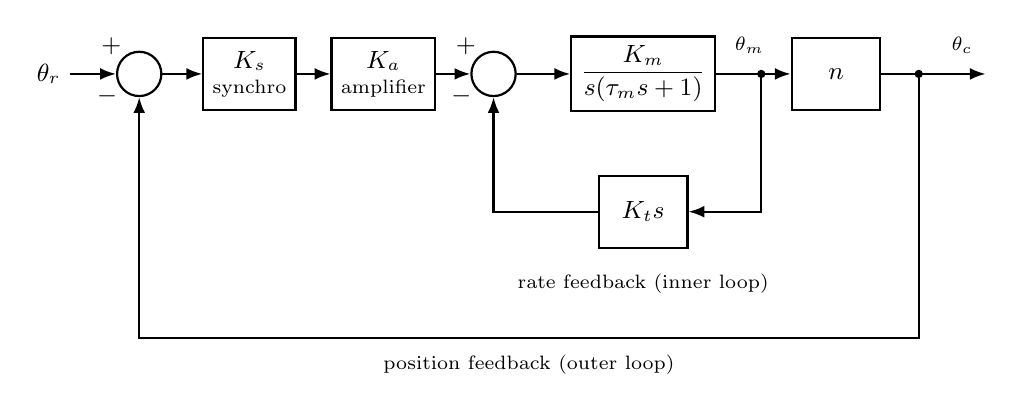
\begin{tikzpicture}[font=\small, x=1cm, y=1cm]
% ---------------- block diagram ----------------
\node (in)  at (0,0) {$\theta_{r}$};
\node[sumnode] (s1) at (1.15,0) {};
\node[block, align=center] (syn) at (2.55,0)
   {$K_{s}$\\[-2pt]{\scriptsize synchro}};
\node[block, align=center] (amp) at (4.25,0)
   {$K_{a}$\\[-2pt]{\scriptsize amplifier}};
\node[sumnode] (s2) at (5.65,0) {};
\node[block, align=center] (mot) at (7.55,0) {$\dfrac{K_{m}}{s(\tau_{m}s+1)}$};
\node[block, align=center] (gear) at (10.0,0) {$n$};
\coordinate (p1) at (9.05,0);
\coordinate (p2) at (11.05,0);
\coordinate (out) at (11.9,0);
\draw[sig] (in) -- (s1);
\draw[sig] (s1) -- (syn);
\draw[sig] (syn) -- (amp);
\draw[sig] (amp) -- (s2);
\draw[sig] (s2) -- (mot);
\draw[sig] (mot) -- (gear);
\draw[sig] (gear) -- (out);
\node[pickoff] at (p1) {};
\node[pickoff] at (p2) {};
\node[font=\scriptsize, anchor=south] at (8.9,0.14) {$\theta_{m}$};
\node[font=\scriptsize, anchor=south] at (11.6,0.14) {$\theta_{c}$};
\sumsign{s1}{135}{+}
\sumsign{s1}{215}{-}
\sumsign{s2}{135}{+}
\sumsign{s2}{215}{-}
% inner tacho loop
\node[block, align=center] (tac) at (7.55,-1.75) {$K_{t}s$};
\draw[sig] (p1) |- (tac.east);
\draw[sig] (tac.west) -| (s2);
\node[font=\scriptsize, anchor=north] at (7.55,-2.42) {rate feedback (inner loop)};
% outer loop
\draw[sig] (p2) -- (11.05,-3.35) -- (1.15,-3.35) -- (s1);
\node[font=\scriptsize, anchor=north] at (6.1,-3.45)
   {position feedback (outer loop)};
\end{tikzpicture}

\vspace{4mm}
% ---------------- step responses ----------------
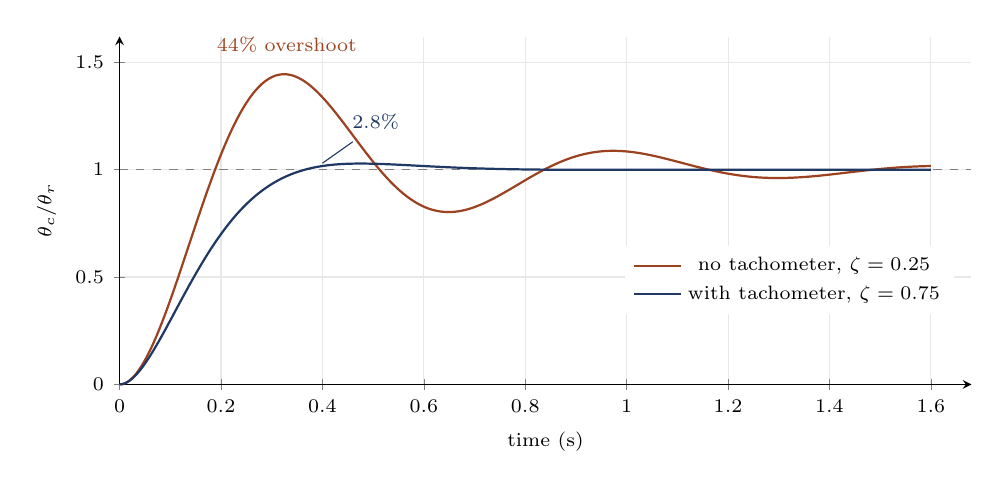
\begin{tikzpicture}
\begin{axis}[
  width=12.4cm, height=6.0cm,
  xlabel={time (s)}, ylabel={$\theta_{c}/\theta_{r}$},
  xlabel style={font=\scriptsize}, ylabel style={font=\scriptsize},
  domain=0:1.6, samples=400,
  xmin=0, xmax=1.68, ymin=0, ymax=1.62,
  ytick={0,0.5,1,1.5}, tick label style={font=\scriptsize},
  grid=both, grid style={gray!18},
  axis lines=left, clip=false,
  legend style={font=\scriptsize, at={(0.98,0.30)}, anchor=east, draw=none},
]
\addplot[thin, gray, dashed, forget plot, domain=0:1.68, samples=2] {1};
\addplot[thick, fflag]
  {1-exp(-2.5*x)*(cos(deg(9.6825*x))+0.2582*sin(deg(9.6825*x)))};
\addlegendentry{no tachometer, $\zt=0.25$}
\addplot[thick, fnavy]
  {1-exp(-7.5*x)*(cos(deg(6.6144*x))+1.1339*sin(deg(6.6144*x)))};
\addlegendentry{with tachometer, $\zt=0.75$}
\node[fflag, font=\scriptsize, anchor=south] at (axis cs:0.33,1.50) {44\% overshoot};
\node[fnavy, font=\scriptsize, anchor=south west] at (axis cs:0.44,1.14) {2.8\%};
\draw[fnavy, thin] (axis cs:0.46,1.13) -- (axis cs:0.40,1.03);
\end{axis}
\end{tikzpicture}
\caption{Rate feedback in a position servo, and what it does. The tachometer
signal never reaches the outer summing junction, so it cannot affect the
steady-state error; it acts only on the motor's effective damping. Both
responses have the same natural frequency and the same final value. Cf.\
Nagrath \& Gopal Fig.~4.14, p.~97.}
\label{fig:ratefb}
\end{figure}

You will meet this idea again as a design tool in Week~9, and study it
properly in FEE3412. Notice one thing about it now, though: the inner loop
feeds back a signal proportional to $s\theta_{m}$ --- the \emph{derivative} of
the output. Anticipating where the output is heading, rather than only where it
is, is what supplies the damping. That is the whole idea behind the derivative
term in a PID controller, met here in hardware before it is met as an
algorithm.

% ====================================================================
\subsection*{Summary of the derivation}

\begin{keyidea}
Each equation in \S\S\ref{sec:actuators}--\ref{sec:tacho}, and where it came
from:
\begin{center}
\begin{tabular}{clP{6.5cm}}
\toprule
Eq. & Result & Origin \\
\midrule
\eqref{eq:torqueconst} & $T_{m}=K_{t}i_{a}$, $K_{t}=zB\ell r$
   & force $B\ell i$ on $z$ conductors at radius $r$ \\
\eqref{eq:emfconst} & $e_{b}=K_{b}\dot\theta$, $K_{b}=zB\ell r$
   & e.m.f.\ $B\ell v$ in the same conductors \\
--- & $K_{t}=K_{b}$
   & power balance $e_{b}i_{a}=T_{m}\dot\theta$ \\
\eqref{eq:dctorquespeed} & $T_{m}=\frac{K_{t}}{R_{a}}v_{a}-\frac{K_{t}K_{b}}{R_{a}}\dot\theta$
   & KVL at steady speed; the slope is damping \\
\eqref{eq:fieldctl} & two lags, no $K_{t}K_{b}$
   & fixing $i_{a}$ removes the back-e.m.f.\ path \\
\eqref{eq:rotfield} & $\mathbf{F}=F_{m}(\cos\omega t,\sin\omega t)$
   & two coils $90^\circ$ apart in space \emph{and} time \\
\eqref{eq:smax} & $s_{\max}=R/X$, $T_{\max}$ independent of $R$
   & maximising \eqref{eq:torqueslip} over slip \\
\eqref{eq:aclin} & $\Delta T_{m}=K\Delta E-f\Delta\dot\theta$
   & first-order Taylor expansion of $T_{m}(\dot\theta,E)$ \\
\eqref{eq:acm} & $K_{m}/[s(\tau_{m}s+1)]$
   & \eqref{eq:aclin} against inertia and friction \\
\eqref{eq:step} & $\alpha=360^\circ/(nT)$
   & stacks offset by one $n$-th of a tooth pitch \\
\eqref{eq:steptorque} & $T_{m}=-Ki^{2}\sin T\theta$
   & $\tfrac{1}{2}i^{2}\,\mathrm{d}L/\mathrm{d}\theta$ with $L=L_{1}+L_{2}\cos T\theta$ \\
\eqref{eq:actacho} & $e_{q}=K_{t}\dot\theta\sin\omega_{c}t$
   & speed voltage in the cup $\to$ quadrature flux $\to$ output coil \\
\eqref{eq:ratefb} & $K_{t}$ only in the $s$ coefficient
   & closing the inner loop before the outer one \\
\bottomrule
\end{tabular}
\end{center}
\end{keyidea}

\subsection*{Check yourself}

\begin{enumerate}[leftmargin=2em,itemsep=2pt]
\item A datasheet gives a motor's torque constant as
      \SI{0.45}{\newton\metre\per\ampere} but does not mention the back-e.m.f.\
      constant. What is it, and how do you know?
\item Why does forcing the armature current constant (field control) destroy
      the motor's electromechanical damping? Answer in terms of
      \eqref{eq:dctorquespeed}, not in terms of the transfer function.
\item Both the synchro stator and the two-phase servomotor stator produce a
      resultant field by adding coil m.m.f.s. One field rotates and the other
      does not. What exactly is different?
\item Show that increasing the rotor resistance of an induction motor does not
      increase its maximum torque. Where does the maximum go instead?
\item A three-stack stepper is required to have a step angle of $2^\circ$.
      How many rotor teeth does it need? A rival design keeps $T=12$ and
      reaches the same step angle by adding stacks instead --- how many stacks
      would that take, and why is it not done that way?
\item In \eqref{eq:ratefb}, what happens to the steady-state output if
      $K_{t}$ is doubled? Explain your answer without computing anything.
\item The reference winding of an a.c.\ tachometer puts the flux $90^\circ$
      behind its excitation, yet the output \eqref{eq:actacho} comes out in
      phase with that excitation. Where did the $90^\circ$ go, and why does it
      matter for a loop that also contains a synchro?
\end{enumerate}

\end{document}

